\documentclass[12pt,a4paper]{report}
\usepackage[utf8]{inputenc}
\usepackage{amsmath}
\usepackage[T1]{fontenc}
\usepackage{lmodern}
\usepackage{amsfonts}
\usepackage{hyperref}
\usepackage{dsfont}
\usepackage{amssymb}
\usepackage[left=1.50cm, right=1.50cm, top=2cm, bottom=2cm]{geometry}
\setlength{\parindent}{0cm}
\usepackage{systeme}
\usepackage{subfigure}
\usepackage{libertine}
\usepackage[pdftex]{graphicx}
\usepackage{tabularx}
\usepackage{xcolor}
\newcommand{\HRule}{\rule{\linewidth}{0.5mm}}
\usepackage[french]{babel}
\usepackage{listings}
\usepackage{amsthm}

\newtheorem{thm}{Théorème}[section]
\newtheorem{definition}{Définition}[section]
\newtheorem{lem}[thm]{Lemme}
\newtheorem{prop}[thm]{Proposition}
\theoremstyle{remark}
\newtheorem*{remark}{Remarque}
\newtheorem*{example}{Exemple}

\begin{document}
\begin{titlepage}
  \begin{sffamily}  
      \flushleft NICOLAS Alexandre \qquad \qquad \qquad \qquad \qquad\qquad \qquad \qquad  \qquad\qquad \qquad \qquad \qquad  MASTER I MIND
      \\DJOUAHRA Sonia \qquad \qquad \qquad    \qquad \qquad \qquad \qquad \qquad \qquad \qquad \qquad \qquad \qquad \qquad \qquad  2020-2021
      \\BERRANDOU Assia 

  \begin{center}
 \textsc{}\\[4cm]
    \textsc{\LARGE Université de Montpellier}\\[2cm]
    \HRule \\[0.4cm]
    { \huge \bfseries Projet : Estimation de paramètres de chaînes de Markov pour modèles d'épidémies\\[0.4cm] }
    \HRule \\[2cm]
    \vspace{4cm}
    \begin{minipage}{1\textwidth}
      \begin{flushleft}
       \includegraphics[scale=0.20]{logo_fds.png}
       \qquad \qquad\qquad\qquad\qquad\qquad\qquad Supervisée par : Mme DE SAPORTA \textsc{Benoîte}\\
       \qquad\qquad\qquad\qquad\qquad\qquad\qquad\qquad\qquad \qquad\qquad \qquad\qquad\qquad\ \ \  Département de Mathématiques
       \end{flushleft}
    \end{minipage}
     \textsc{}\\[1.2cm]
    \vfill
  \end{center}
  \end{sffamily}
\end{titlepage}

\newpage
\section*{Résumé}
\vspace{0.6cm}

Dans ce projet, nous proposons des études mathématiques de différents modèles d'épidémies. C'est à l'aide de modèles Markoviens que nous chercherons par la suite à estimer les paramètres utilisés. Pour ce faire, nous commencerons par construire plusieurs modèles simplifiés de propagation d'épidémie. Nous développerons ensuite des outils d'estimations. A travers cette démarche, nous souhaitons définir des estimateurs et analyser leurs comportements. Ces derniers nous permettrons de déterminer, de façon plus simple, l'évolution de l'épidémie.  

\section*{Remerciements}
\vspace{0.6cm}

Nos remerciements s'adressent tout d'abord à notre responsable de projet Madame Benoîte De Saporta. Nous la remercions pour le temps qu'elle a consacré, sa disponibilité et les précieuses informations qu'elle a apportées pour la réalisation de notre rapport. 
\\
\\
Nous adressons également nos remerciements aux membres du jury et tout particulièrement Monsieur Charlier pour la critique de notre rapport. 

\newpage
\tableofcontents
\newpage
\listoffigures
\newpage
\section*{Introduction}
\vspace{0.6cm}

Une épidémie est définie comme l'apparition et la propagation d'une maladie infectieuse contagieuse qui frappe en même temps et en un même endroit un grand nombre de personnes. De plus, de nos jours, il semble indispensable de s'intéresser à la propagation de cette dernière. Avant toute chose, il serait intéressant de voir sous quelles conditions une épidémie a tendance à se développer ou bien au contraire tendance à s'éteindre. C'est pourquoi nous nous proposons d'étudier, à l'aide des chaînes de Markov, la propagation d'une épidémie.
\\
\\
Un processus de Markov en temps discret est une séquence $(X_n)_{n\in\mathbb{N}}$ de variables aléatoires à valeurs dans l'espace d'états, que l'on notera $E$, et qui possède la propriété de Markov : $X_{n+1}$ ne dépend que de $X_n$, et est donc conditionnellement à $X_n$ indépendante. Le modèle n'a donc pas de "mémoire".
\\
\\
Les chaînes de Markov $(X_n)_{n \in \mathbb{N}}$ , utilisés pour modéliser l'évolution des épidémies, seront construites comme suit. Comme toute la population est observée à chaque pas de temps, nous considérerons une population infinie, où trois événements seront possibles : une contamination, une guérison et une inaction. En effet, un individu est dit contaminé lorsqu'il est infecté par la maladie. A contrario, l'individu est guérie lorsqu'il n'est plus infecté. Une inaction est une absence de contamination et de guérison. 
\\
\\
Nous allons étudier plusieurs modèles qui diffèrent par les probabilités que nous assignerons aux contaminations, guérisons et inactions. Nous regarderons leurs comportements en temps long à l'aide de simulations afin de voir s'il est possible ou non de contrôler l'épidémie.
\\
\\
Dans un dernier temps, nous nous intéresserons aux statistiques de ces chaînes de Markov par l'estimation des paramètres utilisés. Ainsi, nous développerons des outils d'estimations dans plusieurs de ces cas de figure dans le but de connaître les lois sous-jacentes de nos paramètres. 

\newpage
\chapter*{Rappels}

Notre projet s'appuie en majeure partie sur le cours de Processus Stochastiques (cf \cite{cle1}). Le but de ces rappels est de définir les notions de cours utilisées. Il s'agit donc d'un petit guide de relecture.
\\
\\
\begin{definition}
Soit $E$ un ensemble dénombrable, $\mu$ une loi de probabilité sur $E$ et $P$ une matrice stochastique sur $E$. Un processus stochastique $X=(X_n)_{n \in \mathbb{N}}$ est une chaîne de Markov de loi initiale $\mu$ et de matrice de transition $P$ sur $E$ si : \\
i) $X_0$ suit la loi $\mu$, \\
ii) $\forall n \geqslant 0, \, \forall i_0, i_1, ..., i_n \in E, \, \mathbb{P}(X_{n+1}=j|X_n=i, ..., X_0=i_0) = \mathbb{P}(X_{n+1}=j|X_n=i) = p_{ij}.$
\end{definition}
\begin{definition}\label{defa}
On dit que $i$ mène à $j$ et on note $i \longrightarrow j$ s'il existe un entier $n \geq 0$ tel que $\left(P^{n}\right)_{i j}>0$
\end{definition}
\begin{definition}\label{defb}
On dit que $i$ communique $j$ et on note $i \leftrightarrow j$ si i mène à $j$ et $j$ mène a $i$.
\end{definition}
\begin{prop}
La relation de communication est une relation d'équivalence. Les classes d'équivalence sont appelées classes communicantes.
\end{prop}
\begin{definition}\label{def0}
Une classe communicante $C$ est dite fermée si :
$$\forall i \in C, \, \forall j \in E, i \rightarrow j \implies j \in C .$$
\end{definition}
\begin{definition}\label{defa0}
Si la chaîne de Markov a une seule classe de communication, on dit qu'elle est irréductible.
\end{definition}
\begin{definition}\label{def00}
Soit $i$ un état de $E$ et $\mathcal{I}(i)=\left\{n \in \mathbb{N}^{*} ; p_{i i}^{(n)}>0\right\} .$ On appelle période de $i$ le $P G C D$ de l'ensemble $\mathcal{I}(i) .$ Si la période de $i$ est $1$, on dit que $i$ est apériodique. Si $\mathcal{I}(i)=\emptyset$, on dit que la période de $i$ est infinie.
\end{definition}

\begin{thm}\label{th1}
Soit $E$ un ensemble fini ou dénombrable, $U = (U_n)_{n\geq1}$ une suite de variables aléatoires indépendante et de même loi sur $(\mathbb{R},\mathbb{B(R))}$ et $f$ une application mesurable de $E \times \mathbb{R}$ dans $E$. Soit $V$ une variable aléatoire réelle de loi $\mu$ indépendante de 
$U = (U_n)_{n\geq1}$.\\
Alors le processus $X = (X_n)_{n\in \mathbb{N}}$ défini par $X_0=V$ et $X_{n+1}=f(X_{n},U_{n+1})$ est une chaîne de Markov de loi initiale $\mu$ et de matrice de transition $P$ avec $ \forall (i,j) \in E^2, \ \  p_{i,j}=\mathbb{P}(f(i,U_{1})=j).$
\end{thm}

\begin{definition}\label{def1}
Soit $A \subset E$. On appelle temps d'atteinte en $A$ la variable aléatoire : $$T_A = \inf\{{n\geqslant 0} \, ; X_n \in A\}.$$ 
Soit $i \in E$, si $A = \{i\}$, on note : $T_A = T_i$.
\end{definition}

\begin{thm}\label{th2}: Soit $A \subset E$, et $i$ un état de $E$. On note $u_i=\mathbb{P}_i(T_A <\infty)$ la probabilité d'atteindre $A$ en partant de $i$. Soit $u = (u_i , I \in E)$. Alors $u$ est la plus petite solution positive ou nulle du système:
\begin{align*}
 \left\{
\begin{array}{ll}
        u_0=1\\
        u_i= \sum\limits_{j\in E} p_{ij}u_j \ \ \ \forall i \in \mathbb{N}^*
    \end{array}
\right.
\end{align*}
\end{thm}

\begin{definition}\label{def2} 
Soit $A\subset E$. On appelle temps de retour en $A$ la variable aléatoire : $$S_A = \inf\{{n\geqslant 1} \, ; X_n \in A\}.$$
Soit $i \in E$. Si $A = \{i\}$, on note : $S_A = S_i$.
\end{definition}
\begin{definition}\label{defaaa}
Soit $i$ un état de $E$. On dit que $i$ est : 
\begin{itemize}
\item récurrent si  $\mathbb{P}_{i}\left(\exists\right.$ une infinité de $\left.n ; X_{n}=i\right)=1$,
\item transitoire ou transient si  $\mathbb{P}_{i}\left(\exists\right.$ une 
infinité de $\left.n ; X_{n}=i\right)=0$.
\end{itemize}
\end{definition}
\begin{thm}\label{th5}
Tout état de $E$ est soit récurrent, soit transitoire. De plus :
\begin{itemize}
    \item Si $\mathbb{P}_i(S_i<\infty)=1$, alors $i$ est récurrent et $\sum\limits_{n=0}^{\infty} p_{ii}^{(n)}=\infty$
     \item Si $\mathbb{P}_i(S_i<\infty)<1$, alors $i$ est transitoire et $\sum\limits_{n=0}^{\infty} p_{ii}^{(n)}<\infty$
\end{itemize}
On note $p_{i j}^{(n)}=\left(P^{n}\right)_{i j}$ la coordonnée numéro $(i, j)$ de la matrice $P^{n}.$
\end{thm}
\begin{definition}\label{def21}: Soit $X=\left(X_{n}\right)_{n \in \mathbb{N}}$ une chaine de Markov irréductible et récurrente.
\begin{itemize}
    \item Si $\forall i \in E, \, \mathbb{E}_{i}\left[S_{i}\right]<\infty$, on dit que la chaîne est récurrente positive. 
    \item Si $\forall i \in E, \, \mathbb{E}_{i}\left[S_{i}\right]=\infty$, on dit que la chaîne est récurrente nulle.
\end{itemize}
\end{definition}
\begin{thm}\label{th3}
Soit $X=(X_n)_{n \in \mathbb{N}}$ une chaîne de Markov irréductible, récurrente positive et apériodique de probabilité invariante $\pi$. Alors, $\forall (i,j) \in E^2$:
$$\lim\limits_{n \rightarrow \infty} \mathbb{P}_i(X_n = j) = \lim\limits_{n \rightarrow \infty} p^{(n)}_{ij} = \pi_j.$$
\end{thm}

\begin{definition}\label{def3}
Une mesure $\pi$ sur $E$ est une mesure invariante pour la chaîne de Markov
$X=(X_n)_{n \in \mathbb{N}}$ si $\pi P = \pi$. Si $\pi$ est une loi de probabilité, on l'appelle loi invariante de $(X_n)_{n \in \mathbb{N}}$.
\end{definition}
\begin{thm}\label{th6}
Soit $X=(X_n)_{n\in\mathbb{N}}$ une chaîne de Markov irréductible et récurrente. Alors elle possède une unique mesure invariante $\pi$, à constante multiplicative près. De plus, pour tout $i\in E$ on a $0<\pi_i<\infty$ et l'unique mesure invariante $\pi^i$ vérifiant $\pi_i^i=1$ est donnée par $$\pi_j^i = \mathbb{E}_i\left[\sum_{n=0}^{S_i-1}\mathds{1}_j(X_n) \right].$$
C'est donc le nombre moyen de passages en $j$ entre deux passages en $i$.
\end{thm}
\begin{prop}\label{prop1}
: Soit $(X_n)_{n \in \mathbb{N}}$ une chaîne de Markov. Alors, $\forall i \in E$ :
$$\mathbb{P}_i(S_i <\infty) = \sum\limits_{j \in E} \mathbb{P}_j(T_i < \infty) \, \, p_{ij}.$$
\end{prop}
\begin{thm}\label{th61}
Soit $X=\left(X_{n}\right)_{n \in \mathbb{N}}$ une chaine de Markov irréductible et récurrente. Alors elle possède une unique probabilité invariante $\pi$ si et seulement si elle est récurrente positive. Dans ce cas on a
$$
\pi_{i}=\frac{1}{\mathbb{E}_{i}\left[S_{i}\right]}
$$
\end{thm}

\begin{thm}\label{th4}
(ergodique): Soit $X = (X_n)_{n \in \mathbb{N}}$ une chaîne de Markov irréductible récurrente positive de loi invariante $\pi$. Alors, pour toute loi initiale $\mu$ et pour toute fonction $f \, \, \pi$-intégrable :\\
$$\lim\limits_{n \rightarrow \infty}  \frac{1}{n} \sum\limits_{k=0}^{n-1} f\left(X_{k}\right) = \pi f=\sum\limits_{i \in E} f(i) \pi_{i} \, \, \, \, \mathbb{P}_{\mu}-p.s.$$
\end{thm}
\begin{prop}\label{prop0}
Soit $X=\left(X_{n}\right)_{n \in \mathbb{N}}$ une chaine de Markov irréductible et récurrente positive de loi invariante $\pi .$ Alors pour toute loi initiale $\mu$ :
$$
\widehat{p}_{i j}^{n}=\frac{\sum_{k=0}^{n-1} \mathds{1}_{\left(X_{k}=i, X_{k+1}=j\right)}}{\sum_{k=0}^{n-1} \mathds{1}_{\left(X_{k}=i\right)}}
\, \, \, \text{ est un estimateur convergent de } p_{i j}.$$
\end{prop}


\chapter{Modèle d'épidémie simple}

Dans ce premier chapitre, nous allons mettre en place un modèle simple d'épidémie, où les probabilités de contamination, infection et inaction seront constantes par rapport aux nombres de personnes contaminées. Nous étudierons la propagation de l'épidémie à chaque pas de temps en fonction des paramètres choisis. Cette modélisation sera pour nous une première approche de l'analyse du comportement de l'épidémie en temps long.

\section{Construction du modèle}
\vspace{0.6cm}

\begin{definition}\label{def_modele_simple}
On définit $(X_n)_{n\geq0}$ le processus où pour $n$ fixé, $X_n$  représente le nombre d'individus infectés par la maladie à l'instant $n$. Ici, nous choisissons une échelle de temps assez petite par rapport à la dynamique de l'épidémie, pour que le passage de $n$ à $n+1$ correspondent à une personne contaminée ou guérie en plus. 
\\
\\
Soit $(\alpha, \beta, \gamma) \in (\mathbb{R}_+^*)^3$. Il y a donc trois possibilités conditionnellement à $X_n = i, \, \, \forall i \in \mathbb{N}^*$ : 
\\
\begin{itemize}
\item une guérison avec une probabilité $\alpha_i=\frac{\alpha}{\alpha+\beta+\gamma}.$
\item une inaction avec une probabilité $\beta_i=\frac{\beta}{\alpha+\beta+\gamma}.$
\item une contamination avec une probabilité $\gamma_i=\frac{\gamma}{\alpha+\beta+\gamma}.$
\end{itemize}
\vspace{0.5cm}
Pour $i=0$, il ne peut pas y avoir de guérison puisqu'il n'y a aucune personne infectée. Nous avons alors :
\\
\begin{itemize}
\item une inaction avec une probabilité $1-\gamma_0=\alpha_0 + \beta_0 = \frac{\alpha + \beta}{\alpha+\beta+\gamma}.$
\item une contamination avec une probabilité $\gamma_0=\frac{\gamma}{\alpha+\beta+\gamma}.$
\end{itemize}
\vspace{0.5cm}

Notons que, dans ce modèle, les probabilités ne dépendent pas de $i$. Nous supposons que $X_{0} = 0$ et nous avons donc :
\begin{itemize}
\item $\forall n \in \mathbb{N}$, \, si $X_n=0$,\, alors $X_{n+1} = \left\{
    \begin{array}{ll}
        X_n+1 & \mbox{si le (n+1)ème événement est une contamination } \\
        X_n & \mbox{sinon. }
    \end{array}
\right. $
\item $\forall n \in \mathbb{N}^*$, \, si $X_n > 0$,\, alors $X_{n+1} = \left\{
    \begin{array}{ll}
        X_n+1 & \mbox{si le (n+1)ème événement est une contamination} \\
        X_n-1 & \mbox{si le (n+1)ème événement est une guérison} \\
        X_n & \mbox{sinon. }\\
    \end{array}
\right. $
\end{itemize}
\end{definition}

\begin{prop}\label{simple_markov}
Le processus $(X_n)_{n \in \mathbb{N}}$ est une chaîne de Markov de loi initiale $\delta_0$ et de matrice de transition :
$$P=
\begin{pmatrix}
        1-\gamma_0 & \gamma_0 & 0 & 0 & \cdots \\ 
         \alpha_1 & \beta_1 & \gamma_1 & 0 & \cdots\\
         0 & \alpha_2 & \beta_2 & \gamma_2 & \cdots\\
        \vdots &\ddots & \ddots & \ddots & \ddots \\ 
\end{pmatrix}$$
\end{prop}
\begin{proof}
Soit $(U_n)_{n\in \mathbb{N}}$ une suite de variables aléatoires indépendantes à valeurs dans $\{-1, 0, 1\}$ telles que $\forall n \in \mathbb{N}$: \\
\begin{itemize}
    \item $\mathbb{P}(U_n=1)= \frac{\gamma}{\alpha+\beta+\gamma},$
    \item $\mathbb{P}(U_n=0)= \frac{\beta}{\alpha+\beta+\gamma},$
    \item $\mathbb{P}(U_n=-1)= \frac{\alpha}{\alpha+\beta+\gamma}.$
\end{itemize}

\vspace{0.7cm}
On peut donc écrire : 
$$\forall n \in \mathbb{N}, \ \ \ X_{n+1} = (X_n + U_{n+1}) \mathds{1}_{(X_n >0)} + \mathds{1}_{(X_n=0)}\mathds{1}_{(U_{n+1}=1)}.$$

Soit $E=\mathbb{N}$. On définit l'application  : 
\begin{center}
$\begin{array}{ccccc}
h & : & E \times \mathbb{R} & \longrightarrow & \mathbb{R} \\
 & & (\ x \ ,\ y\ ) & \mapsto & (x + y) \mathds{1}_{(x >0)} + \mathds{1}_{(x=0)}\mathds{1}_{(y=1)}\\
\end{array}.$
\end{center}
 
\vspace{0.3cm}
L'application $h$ est une fonction mesurable, $(U_n)_{n\in\mathbb{N}}$ une suite de variables aléatoires i.i.d à valeurs dans ($\mathbb{R},\cal{B}(\mathbb{R})$), $X_0$ une variable aléatoire à valeurs dans $E$ et indépendante de $(U_n)_{n\in \mathbb{N}}$ et $\forall n \in \mathbb{N}, \ \\X_{n+1}=h(X_n;U_{n+1})$.
\\
\\
Alors, par le théorème \ref{th1}, le processus $(X_n)_{n\in\mathbb{N}}$ défini par $X_0 = 0$ et $X_{n+1}=h(X_n,U_{n+1})$ est une chaîne de Markov de loi initiale $\delta_0$ et de matrice de transition $P = (p_{ij})_{(i,j) \in E^2}$ avec $p_{ij} = \mathbb{P}(h(i, U_{n+1} = j)$. 
\end{proof}
\vspace{0.5cm}

La figure $1.1$ représente le graphe orienté associé à la chaîne de Markov. Nous pouvons, à partir de ce graphe, déterminer les classes communicantes de $(X_n)_{n \in \mathbb{N}}.$

\begin{figure}[h]
    \centering
    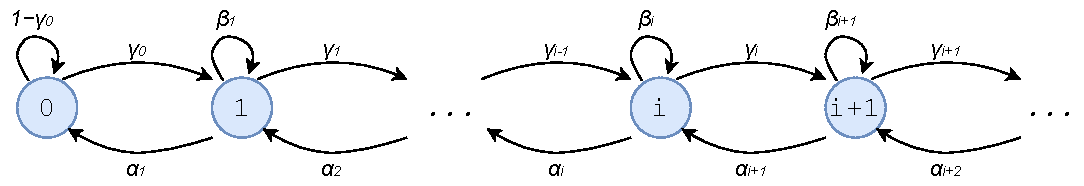
\includegraphics[scale=1]{graphe_model_simple.pdf} 
    \caption{Graphe orienté du modèle simple d'épidémie}
    \label{fig:my_label}
\end{figure}

\begin{remark}
On a : $\forall i \in \mathbb{N},\ \  i \longleftrightarrow i+1$.
Il y a donc une seule classe fermée $C=\mathbb{N}$. Vu que l'espace d'états est de cardinal infini, cette dernière peut être transitoire ou récurrente. Nous étudierons en détail la nature de la chaîne dans la partie suivante. Regardons avant cela la période de la classe.
\end{remark}

\begin{prop}\label{aperiodique}
La chaîne de Markov $(X_n)_{n \in \mathbb{N}}$ est apériodique.
\end{prop}
\begin{proof}
Soit $i \in \mathbb{N}$ et $I(i) = \{n \in \mathbb{N}^* \, \, | \, \,p_{ii}^{(n)} > 0\}$. Nous avons $p_{11}^{(1)} = \beta_1 > 0$, d'où : $1 \in I(1)$. $1$ est donc de période $1$ et par propriété de classe, $\forall i \in \mathbb{N}$, $i$ est de période $1$. Ainsi, $(X_n)_{n \in \mathbb{N}}$ est apériodique.
\end{proof}

\section{Classification du processus}

\subsection{Évaluation de la propagation de l'épidémie}
\vspace{0.6cm}

Dans cette section, nous allons désormais calculer la probabilité d'atteindre $0$ infecté. Notons que même en atteignant $0$, l'épidémie pourrait redémarrer. Il s'agit donc de voir s'il est possible de la contrôler ou non.
\begin{thm}
Soit $T_0$ le temps d'atteinte en $0$. Soit $i \in \mathbb{N}$. On pose $u_i=\mathbb{P}_i(T_0 < \infty)$ et $u=(u_i,\  i\in \mathbb{N})$. Alors :
\begin{itemize}
    \item Si $\alpha \geqslant \gamma$, alors $\forall i \in \mathbb{N}, \, \, u_i = 1$
    \item  Si $\alpha < \gamma$, alors $\forall i \in \mathbb{N}, \, \, u_i = \left(\frac{\alpha}{\gamma}\right)^i$
\end{itemize}
\end{thm}
\begin{proof}
Par le théorème \ref{th2}, $u$ est la plus petite solution positive ou nulle du système : 
$$(S) : \left\{
\begin{array}{ll}
        u_0=1,\\
        u_i= \sum\limits_{j\in E} p_{ij}u_j \ \ \ \forall i \in \mathbb{N}^*.
    \end{array}
\right.$$
Notons tout d'abord que : $\beta_i-1 = \frac{\beta}{\alpha+\beta+\gamma}-1 = \frac{-(\alpha+\gamma)}{\alpha+\beta+\gamma} = -(\alpha_i+\gamma_i).$ Nous pouvons alors résoudre le système :
\begin{align*}
(S) &\Longleftrightarrow  \left\{
\begin{array}{ll}
        u_0=1\\
        u_i= \alpha_i u_{i-1} + \beta_i u_i + \gamma_i u_{i+1} \ \ \ \forall i \in \mathbb{N}^*
    \end{array}
\right.  \\
&\Longleftrightarrow \left\{
\begin{array}{ll}
        u_0=1\\
        \alpha_i u_{i-1} + (\beta_i-1) u_i + \gamma_i u_{i+1} = 0 \ \ \ \forall i \in \mathbb{N}^*
    \end{array}
\right.  \\
 &\Longleftrightarrow \left\{
\begin{array}{ll}
        u_0=1\\
        \alpha_i u_{i-1} - (\alpha_i+\gamma_i) u_i + \gamma_i u_{i+1} = 0 \ \ \ \forall i \in \mathbb{N}^*
    \end{array}
\right.  \\
 &\Longleftrightarrow \left\{
\begin{array}{ll}
        u_0=1\\
        \alpha u_{i-1} - (\alpha+\gamma) u_i + \gamma u_{i+1} = 0 \ \ \ \forall i \in \mathbb{N}^*.
    \end{array}
\right. 
\end{align*}

\vspace{0.5cm}

Nous avons une suite récurrente linéaire d'ordre 2. Le polynôme associé est  : $\gamma X^2 -(\alpha+\gamma)X+\alpha$. Cherchons les racines de ce polynôme. Le discriminant est :
\begin{align*}
\Delta &= (-(\alpha+\gamma))^2 - 4\gamma \alpha \\
&=\alpha^2 + \gamma^2-2\gamma\alpha \\
&= (\alpha-\gamma)^2.
\end{align*}

\textbf{\underline{Cas 1} :} Si $\alpha = \gamma$, alors $\Delta = 0$. Il y a donc une seule solution réelle : 
$$x = \frac{\alpha + \gamma}{2 \gamma}=  \frac{2\gamma}{2\gamma} = 1.$$

Les solutions sont donc de la forme $\forall i \in \mathbb{N}, u_i = (a+ib) \, x^i = a+ib$.\\
$$(S) \iff \left\{
\begin{array}{ll}
        u_0=1\\
        u_i=a+ib \ \ \forall i \in \mathbb{N}
    \end{array}
\right. 
\iff \left\{
\begin{array}{ll}
        u_0=a=1\\
        u_i=a+ib \ \ \forall i \in \mathbb{N}
    \end{array}
    \right. 
\iff \left\{
\begin{array}{ll}
        a = 1\\
        u_i=1+ib \ \ \forall i \in \mathbb{N}.
    \end{array}
    \right.$$
\\
Or, vu que $u$ est la plus petite solution positive du système, on a $b=0$.\\
Donc : $\forall i \in \mathbb{N}, \, u_i=1.$
\vspace{0.7cm}\\
\textbf{\underline{Cas 2} :} Si $\alpha \neq \gamma$, alors $\Delta > 0$. Il y a alors deux solutions réelles : 
\\
\begin{itemize}
\item $x_1 = \frac{\alpha + \gamma - (\alpha-\gamma)}{2\gamma}=\frac{2\gamma}{2\gamma}=1.$
\item $x_2= \frac{\alpha + \gamma + \alpha-\gamma}{2\gamma}=\frac{2\alpha}{2\gamma}=\frac{\alpha}{\gamma}.$
\end{itemize}
\vspace{0.5cm}
Les solutions sont donc de la forme $\forall i \in \mathbb {N}, u_i = a \times 1^i + b \times (\frac{\alpha}{\gamma})^i = a+b\times (\frac{\alpha}{\gamma})^i$ avec $(a,b) \in \mathbb{R}^2$. Nous avons alors :
\\
\begin{align*}
(S) &\iff \left\{
\begin{array}{ll}
        u_0=1\\
        u_i=a+b\times \left(\frac{\alpha}{\gamma}\right)^i  \ \ \forall i \in \mathbb{N}
    \end{array}
\right. 
\iff \left\{
\begin{array}{ll}
        a+b=1\\
        u_i=a+b\times \left(\frac{\alpha}{\gamma}\right)^i \ \ \forall i \in \mathbb{N}
    \end{array}
\right. \\
&\iff \left\{
\begin{array}{ll}
        a=1-b\\
        u_i=1-b+b\times \left(\frac{\alpha}{\gamma}\right)^i \ \ \forall i \in \mathbb{N}
    \end{array}
\right.
\iff \left\{
\begin{array}{ll}
        a=1-b\\
        u_i=1+b \, \left(\left(\frac{\alpha}{\gamma}\right)^i - 1\right)\ \ \forall i \in \mathbb{N}.
    \end{array}
\right.
\end{align*}

- Si $\alpha < \gamma$, alors $\frac{\alpha}{\gamma} < 1$, d'où : $-1 < \left(\frac{\alpha}{\gamma}\right)^i - 1 < 0$. Vu que $u$ est la plus petite solution positive du système, nous avons nécessairement $b = 1$, d'où : $\forall i \in \mathbb{N}, \, u_i = \left(\frac{\alpha}{\gamma}\right)^i$.\\

- Si $\alpha > \gamma$, alors $\frac{\alpha}{\gamma} > 1$, d'où : $\left(\frac{\alpha}{\gamma}\right)^i - 1 > 0$. Vu que $u$ est la plus petite solution positive du système, nous avons nécessairement $b = 0$, d'où : $\forall i \in \mathbb{N}, \, u_i =1$.
\end{proof}

Les résultats obtenus sont cohérents. En effet, $\alpha$ correspond au taux de guérison et $\gamma$ à celui de contamination. Si le taux de guérison est plus élevé que celui de contamination, nous sommes sûrs d'atteindre l'état $0$ partant de n'importe quel état et l'épidémie sera contrôlée. A l'inverse, si le taux de guérison est inférieur à celui de contamination, nous avons $\lim\limits_{i \to +\infty} u_i = 0$. Cela signifie qu'il est de plus en plus difficile d'endiguer l'épidémie si le nombre d'infectés est trop élevé.
\\
\subsection{Nature du processus}
\vspace{0.6cm}

Vu que la chaîne de Markov est irréductible, nous souhaitons étudier sa nature, c'est-à-dire savoir si elle est récurrente ou transitoire. Étant donné que nous travaillons avec un espace d'états non fini, nous ne pouvons pas déterminer directement la nature de la chaîne. Nous allons de ce fait utiliser le théorème \ref{th5}.

\begin{prop}
Nous avons les deux cas de figure suivants :
\begin{itemize}
    \item Si $\alpha < \gamma$, alors $(X_n)_{n \in \mathbb{N}}$ est transitoire.
    \item Si $\alpha \geqslant \gamma$, alors $(X_n)_{n \in \mathbb{N}}$ est récurrente.
\end{itemize}
\end{prop}
\begin{proof}
\textbf{\underline{Cas 1} :} Si $\alpha<\gamma$, nous avons : 
\begin{align*}
\mathbb{P}_0(S_0 < \infty) &= \sum_{j\in E}{\ \mathbb{P}_j(T_0 < \infty)p_{0j}} \\
&= (1-\gamma_{i}) \times 1 + \gamma_{i} \times \frac{\alpha}{\gamma} \\
&=\frac{\alpha+\beta}{\alpha+\beta+\gamma}+\frac{\alpha}{\alpha+\beta+\gamma} \\
&= \frac{2\alpha+\beta}{\alpha+\beta+\gamma}
\end{align*}

Or, $\alpha < \gamma$, ce qui implique $2\alpha + \beta < \alpha + \beta + \gamma$, d'où : $\frac{2\alpha+\beta}{\alpha+\beta+\gamma} < 1$. Nous obtenons ainsi que $\mathbb{P}_0(S_0 < \infty) < 1$. \\
Par le théorème \ref{th5}, l'état $0$ est transitoire. Par propriété  de classe, la classe $C$ est transitoire, et donc $(X_n)_{n \in \mathbb{N}}$ est transitoire.\\

\textbf{\underline{Cas 2} :} Si $\alpha \geqslant \gamma$, alors $u_i=1$. Nous avons alors :
$$\mathbb{P}_0(S_0 < \infty)=
 1-\gamma_i+\gamma_i=1.$$

Par le théorème \ref{th5}, l'état $0$ est récurrent, et par propriété de classe, $(X_n)_{n \in \mathbb{N}}$ est récurrente.
\end{proof}

Nous avons donc deux possibilités. Si le taux d'infection est strictement supérieur au taux de guérison, le nombre de contaminés aura tendance à augmenter plutôt que diminuer entre les temps $n$ et $n+1$, ce qui entraînera une forte propagation de l'épidémie. A long terme, le nombre de contaminé tend vers $+\infty$. Si le taux de guérison $\alpha$ est supérieur ou égal au taux  d'infection $\gamma$, un individu contaminé aura tendance à guérir plus rapidement que le virus ne se propage. La propagation de l'épidémie sera donc freinée par les guérisons plus rapides et nous visiterons toutes les valeurs, y compris très grandes, avec probabilité 1.
\\
\subsection{Le cas récurrent}
\vspace{0.6cm}

Intéressons nous désormais de plus près au cas où la chaîne est récurrente, c'est-à-dire lorsque $\alpha \geqslant \gamma$. Nous souhaitons déterminer si la chaîne est récurrente nulle ou récurrente positive selon les valeurs des paramètres. 

\begin{prop}\label{nulle_positive}
Nous avons les deux possibilités suivantes :
\begin{itemize}
    \item  Si $\alpha = \gamma$, alors $(X_n)_{n \in \mathbb{N}}$ est récurrente nulle.
    \item Si $\alpha > \gamma$, alors $(X_n)_{n \in \mathbb{N}}$ est récurrente positive.
\end{itemize}
\end{prop}
\begin{proof}
Vu que la chaîne est irréductible, d'après le théorème \ref{th6}, $(X_n)_{n\in\mathbb{N}}$ admet une unique mesure invariante $\pi=(\pi_i\, , \, i \in E)$ à une constante multiplicative près et $\forall i \in E, \, \, \, 0< \pi_i<\infty$. Calculons :
\begin{align*}
\pi P=\pi
&\iff (\pi_0,\pi_1,...) \begin{pmatrix}
        1-\gamma_0 & \gamma_0 & 0 & 0 & \cdots \\ 
         \alpha_1 & \beta_1 & \gamma_1 & 0 & \cdots\\
         0 & \alpha_2 & \beta_2 & \gamma_2 & \cdots\\
        \vdots &\ddots & \ddots & \ddots & \ddots \\ 
\end{pmatrix} = (\pi_0,\pi_1,...)\\
&\iff 
\left\{
\begin{array}{ll}
        \pi_0=(1-\gamma_0)\pi_0+\alpha_1\pi_1 \\
        \pi_i=\gamma_{i-1}\pi_{i-1}+\beta_{i}\pi_{i}+\alpha_{i+1}\pi_{i+1} \, \, \, \forall i \in \mathbb{N}^*
    \end{array}
\right. \\
&\iff \left\{
\begin{array}{ll}
         \gamma_0\pi_0=\alpha_1\pi_1 \\
        \gamma_{i-1}\pi_{i-1}+(\beta_{i}-1)\pi_{i}+\alpha_{i+1}\pi_{i+1} = 0 \, \, \, \forall i \in \mathbb{N}^*
    \end{array}
\right. \\
&\iff \left\{
\begin{array}{ll}
         \gamma\pi_0=\alpha\pi_1 \\
        \gamma\pi_{i-1}-(\alpha+\gamma)\pi_{i}+\alpha\pi_{i+1} = 0 \, \, \, \forall i \in \mathbb{N}^*
    \end{array}
\right. \\
&\iff \left\{
\begin{array}{ll}
         \pi_0=\frac{\alpha}{\gamma}\pi_1 \\
        \gamma\pi_{i-1}-(\alpha+\gamma)\pi_{i}+\alpha\pi_{i+1} = 0 \, \, \, \forall i \in \mathbb{N}^*.
    \end{array}
\right.
\end{align*}

Nous avons une suite récurrente linéaire d'ordre 2. Le polynôme associé est  : $\alpha X^2 -(\alpha+\gamma)X+\gamma$. Nous retrouvons le même discriminant que précédemment.

\vspace {0.5cm}
\textbf{\underline{Cas 1 } :} Si $\alpha = \gamma$, alors $\Delta = 0$. Il y a donc une seule solution réelle : $x =1.$
Les solutions sont donc de la forme : $\forall i \in \mathbb{N}, \pi_i = (a+ib) \, x^i = a+ib$. Nous avons alors : $$
\left\{
\begin{array}{ll}
        \pi_0 = a\\
        \pi_1 = a + b
    \end{array}
\right. 
\iff \left\{
\begin{array}{ll}
        a = \frac{\alpha}{\gamma}\pi_1\\
        \pi_1 = a + b
    \end{array}
    \right. 
\iff \left\{
\begin{array}{ll}
       a = \pi_1\\
       \pi_1 = \pi_1 + b\\
    \end{array}
    \right.
\iff \left\{
\begin{array}{ll}
       a = \pi_1\\
      b = 0 .\\
\end{array}
\right.
$$
\\
Nous en déduisons : $\forall i \in \mathbb{N}, \, \pi_i = \pi_1$, i.e $\pi = c (1,1,1,...)$ avec $c \in \mathbb{R}_+^*$.
\\
\\
Soit $i \in \mathbb{N}$, et $\pi^i$ l'unique mesure invariante vérifiant $\pi_i^i=1$. Nous notons $c_i\in \mathbb{R}_+^*$ la constante telle que $\pi_i^i=1$. Ici, nous avons : $\pi^i=c_i\left(1,1,...,1,...\right)=\left(1,1,...,1,...\right)$.
Alors, par le théorème \ref{def21}, $\forall i \in E$ :
$$\mathbb{E}_i[S_i]=\sum\limits_{j\in E }\pi_j^i = \sum\limits_{j\in\mathbb{N} }1 = +\infty.$$

Ainsi, pour $\alpha=\gamma$, $(X_n)_{n\in\mathbb{N}}$ est récurrente nulle.
\\
\\
\textbf{\underline{Cas 2 } :} Si $\alpha > \gamma$, alors $\Delta > 0$. Il y a alors deux solutions réelles : $x_1= \frac{\gamma}{\alpha}$ et $x_2=1.$
\\
\\
Les solutions sont donc de la forme $\forall i \in \mathbb {N}, \pi_i = a \times 1^i + b \times (\frac{\gamma}{\alpha})^i = a+b\times (\frac{\gamma}{\alpha})^i$ avec $ (a,b) \in \mathbb{R}^2$.

Alors :
\begin{align*}
&\left\{
\begin{array}{ll}
  \pi_0 = a + b\\
  \pi_1 = a + b \times \left(\frac{\gamma}{\alpha}\right) 
    \end{array}
\right. 
\iff \left\{
\begin{array}{ll}
  \frac{\alpha}{\gamma}\pi_1 = a + b\\
  \pi_1 = a + b \times \left(\frac{\gamma}{\alpha}\right) 
    \end{array}
\right. 
\iff \left\{
\begin{array}{ll}
  b=\frac{\alpha}{\gamma}\pi_1-a\\
  \pi_1=a+(\frac{\alpha}{\gamma}\pi_1-a)\times \frac{\gamma}{\alpha}
    \end{array}
\right.\\
\iff &\left\{
\begin{array}{ll}
         b=\frac{\alpha}{\gamma}\pi_1-a\\
        \pi_1=a+\pi_1-a \frac{\gamma}{\alpha}
    \end{array}
\right. 
\iff \left\{
\begin{array}{ll}
        b=\frac{\alpha}{\gamma}\pi_1-a\\
        a \times(1-\frac{\gamma}{\alpha}) = 0 .
    \end{array}
\right.
\end{align*}

Comme $\alpha>\gamma$, on a $\frac{\gamma}{\alpha}\neq1 \Rightarrow (1-\frac{\gamma}{\alpha})\neq 0$.
D'où $a=0 $ et $b = \frac{\alpha}{\gamma}\pi_1$. Nous en déduisons :
$$\forall i \in \mathbb{N}, \, \pi_i =  \frac{\alpha}{\gamma}\pi_1 \times  \left(\frac{\gamma}{\alpha}\right)^i =\pi_1\left(\frac{\gamma}{\alpha}\right)^{i-1}.$$

Nous reprenons les notations précédentes et nous obtenons $\forall i \in \mathbb{N}$ :
$\pi^i = c_i \left(\frac{\alpha}{\gamma},\frac{\gamma}{\alpha},...,\frac{\gamma}{\alpha}^{i},...\right)$ avec $c_i \in\mathbb{R}_+^*.$

Alors : $c_0 = \frac{\gamma}{\alpha}$ et $\forall i \in \mathbb{N}, \, c_i = \left(\frac{\alpha}{\gamma}\right)^i$. Calculons $\forall i \in \mathbb{N}$ l'espérance partant de $i$ du temps de retour en $i$ :
$$\mathbb{E}_i[S_i] = \sum\limits_{j\in E }\pi_j^i = \sum\limits_{j\in \mathbb{N} }c_i \left(\frac{\gamma}{\alpha}\right)^{j-1} = c_i \,  \frac{\alpha}{\gamma} \, \sum\limits_{j = 0 }^{+\infty} \left(\frac{\gamma}{\alpha}\right)^{j}.$$
\\
Or : $\alpha > \gamma \implies \frac{\gamma}{\alpha} < 1$. Nous avons donc une série géométrique de premier terme $1$ et de raison $q = \frac{\gamma}{\alpha} < 1$. La série est donc convergente. Calculons :
$$\mathbb{E}_i[S_i] = c_i \,  \frac{\alpha}{\gamma} \, \frac{1}{1 - \frac{\gamma}{\alpha}} = c_i \,  \frac{\alpha}{ \frac{\gamma \alpha - \gamma^2}{\alpha}} = c_i \,  \frac{\alpha^2}{\gamma(\alpha - \gamma)}.$$
\\
Pour $i = 0$ : $$\mathbb{E}_0[S_0] = c_0 \,  \frac{\alpha^2}{\gamma(\alpha - \gamma)} = \frac{\gamma}{\alpha}  \,  \frac{\alpha^2}{\gamma(\alpha - \gamma)} = \frac{\alpha}{\alpha - \gamma} < +\infty.$$
\\
Pour $i \geqslant 1$ : $$\mathbb{E}_i[S_i] = c_i \,  \frac{\alpha^2}{\gamma(\alpha - \gamma)} = \left(\frac{\alpha}{\gamma}\right)^i  \,  \frac{\alpha^2}{\gamma(\alpha - \gamma)} = \frac{\alpha^{i+2}}{\gamma^{i+1}(\alpha - \gamma)} < +\infty.$$
\\
\\
Finalement : $\forall i \in \mathbb{N}, \, \, \mathbb{E}_i[S_i] < +\infty$. Ainsi, pour $\alpha > \gamma, \, \, (X_n)_{n \in \mathbb{N}}$ est récurrente positive.
\end{proof}
Dans le cas où $(X_n)_{n \in \mathbb{N}}$ est irréductible et récurrente positive, le théorème \ref{th61} nous dit que la chaîne admet une unique loi invariante $\pi$. Cette dernière est donnée par la proposition suivante.
\begin{prop}
La loi invariante $\pi$ de $(X_n)_{n \in \mathbb{N}}$ est donnée par :
\begin{itemize}
    \item $\pi_0 = \frac{\alpha - \gamma}{\alpha}$
    \item Pour $i \geqslant 1, \, \, \pi_i = \frac{\gamma^{i+1}(\alpha - \gamma)}{\alpha^{i+2}}$
\end{itemize}
\end{prop}
\begin{proof}
Le théorème \ref{th61} implique qu'il existe une constante $c$ tel que $c\pi$ soit une loi de probabilité et nous avons $\forall i \in \mathbb{N}$ : 
$$\pi_i = \frac{1}{\mathbb{E}_i[S_i]}.$$
\\
En utilisant les résultats de la preuve de la proposition \ref{nulle_positive}, nous obtenons :
\\
\\
Pour $i = 0$ : $$\pi_0 = \frac{1}{\mathbb{E}_0[S_0]} = \frac{\alpha - \gamma}{\alpha}.$$
\\
Pour $i \geqslant 1$ : $$\pi_i = \frac{\gamma^{i+1}(\alpha - \gamma)}{\alpha^{i+2}}.$$
\end{proof}

\begin{prop}
$\forall (i,j) \in \mathbb{N}^2$, nous avons : $\lim\limits_{n \to +\infty} \mathbb{P}_i(X_n = j) = \pi_j.$
\\
\\
En particulier : $\forall i \in \mathbb{N}^*, \, \, \lim\limits_{n \to +\infty} \mathbb{P}_i(X_n = 0) = \pi_0 = \frac{\alpha - \gamma}{\alpha}.$
\end{prop}
\begin{proof}
D'après le théorème \ref{th61} et la proposition \ref{aperiodique}, $(X_n)_{n \in \mathbb{N}}$ est une chaîne de Markov irréductible récurrente positive et apériodique de probabilité invariante $\pi$. Le théorème \ref{th3} nous donne directement le résultat.
\end{proof}

Ainsi, la probabilité partant de n'importe quel état différent de $0$ d'atteindre $0$ à long terme est de $\frac{\alpha - \gamma}{\alpha}$.

\subsection{Ergodicité}
\vspace{0.6cm}

Le but de cette partie va être d'appliquer le théorème ergodique, théorème \ref{th4},  à notre chaîne de Markov dans le cas où cette dernière est récurrente positive, afin de déterminer le nombre d'infectés moyen à long terme $\lim\limits_{n \to +\infty} \frac{1}{n} \sum\limits_{k=0}^{n-1} X_k$. Nous sommes donc dans le cas où $\alpha > \gamma$.

\begin{thm}
Le nombre moyen d'infectés à long terme est égal à $\frac{\gamma^2}{\alpha^2-\gamma^2}$.
\end{thm}
\begin{proof}
Soit $f : \mathbb{N} \longrightarrow \mathbb{N}$, la fonction identité, i.e $\forall i \in \mathbb{N}, \, \, f(i) = i$. Nous avons :
$$\sum\limits_{i \in \mathbb{N}} |f(i)| \pi_i = \sum\limits_{i = 0}^{+\infty} i \, \, \pi_i = \sum\limits_{i = 1}^{+\infty} i \, \, \frac{\gamma^{i+1}(\alpha - \gamma)}{\alpha^{i+2}} = \frac{\alpha - \gamma}{\alpha} \, \, \sum\limits_{i = 1}^{+\infty} i \, \, \left(\frac{\gamma}{\alpha}\right)^{i+1}.$$
\\
Posons : $A = \sum\limits_{i = 1}^{+\infty} i \, \, \left(\frac{\gamma}{\alpha}\right)^{i+1}$. Alors :

$$A = \sum\limits_{i = 1}^{+\infty} (i - 1 + 1) \, \, \left(\frac{\gamma}{\alpha}\right)^{i+1} \\
= \sum\limits_{i = 1}^{+\infty} (i - 1) \, \, \left(\frac{\gamma}{\alpha}\right)^{i+1} + \sum\limits_{i = 1}^{+\infty}  \left(\frac{\gamma}{\alpha}\right)^{i+1}.$$
\\
Nous faisons le changement d'indices suivant : $j = i - 1$. Nous avons alors, si $i=1, j=0 \, \,$ et si $i$ tend vers $+\infty$, $j$ tend vers $+ \infty$. Nous obtenons alors :
\\
$$A = \sum\limits_{j = 0}^{+\infty} j \, \, \left(\frac{\gamma}{\alpha}\right)^{j+2} + \frac{\gamma}{\alpha} \, \, \sum\limits_{i = 1}^{+\infty}  \left(\frac{\gamma}{\alpha}\right)^{i} = \left(\frac{\gamma}{\alpha}\right)^2 \times A + \left(\frac{\gamma}{\alpha}\right)^2 \times \frac{1}{1 - \frac{\gamma}{\alpha}}.$$
\begin{align*}
&\Rightarrow A\left(1-\left(\frac{\gamma}{\alpha}\right)^2\right) = \left(\frac{\gamma}{\alpha}\right)^2 \times \frac{\alpha}{\alpha-\gamma} = \frac{\gamma^2}{\alpha\left(\alpha-\gamma\right)}\\
&\Rightarrow A = \frac{\alpha^2}{\alpha^2-\gamma^2}\times \frac{\gamma^2}{\alpha\left(\alpha-\gamma\right)}=\frac{\alpha}{\alpha^2-\gamma^2}\times \frac{\gamma^2}{\left(\alpha-\gamma\right)}.
\end{align*}
D'où : 
$$\sum\limits_{i \in \mathbb{N}} |f(i)| \pi_i =\frac{\alpha-\gamma }{\alpha} \times \frac{\alpha}{\alpha^2-\gamma^2}\times \frac{\gamma^2}{\left(\alpha-\gamma\right)} = \frac{\gamma^2}{\alpha^2-\gamma^2}< +\infty .$$
\\
Donc : $f$ est $\pi$-intégrable.\\

D'après le théorème \ref{th61}, le processus $(X_n)_{n\in\mathbb{N}}$ est une chaîne de Markov irréductible et récurrente positive de loi invariante $\pi$. De plus, $f$ est $\pi$-intégrable. Alors, d'après le théorème \ref{th4}, pour toute loi initiale $\mu$ : 
$$\lim\limits_{n \to +\infty} \frac{1}{n} \sum\limits_{k=0}^{n-1} X_k= \pi f = \sum\limits_{i\in\mathbb{N}} f(i)\pi_i= \frac{\gamma^2}{\alpha^2-\gamma^2} \text{   }\, \, \, \mathbb{P}_{\mu}-p.s.$$
\end{proof}

Ainsi, à long terme, le nombre moyen d'infectés dépend de $\alpha$ et $\gamma$ et est égal à $\frac{\gamma^2}{\alpha^2-\gamma^2}$.

\section{Simulations}
\vspace{0.6cm}

Pour terminer l'étude du modèle simple d'épidémie, nous avons simulé le comportement de notre chaîne de Markov en fonction des différents taux $\alpha, \beta$ et $ \gamma$. Nous observons son comportement pour une durée de $n=1000$. Nous obtenons alors les graphiques de la figure suivants. \\
\begin{figure}[h!]
    \begin{minipage}[c]{0.25\linewidth}
        \centering
        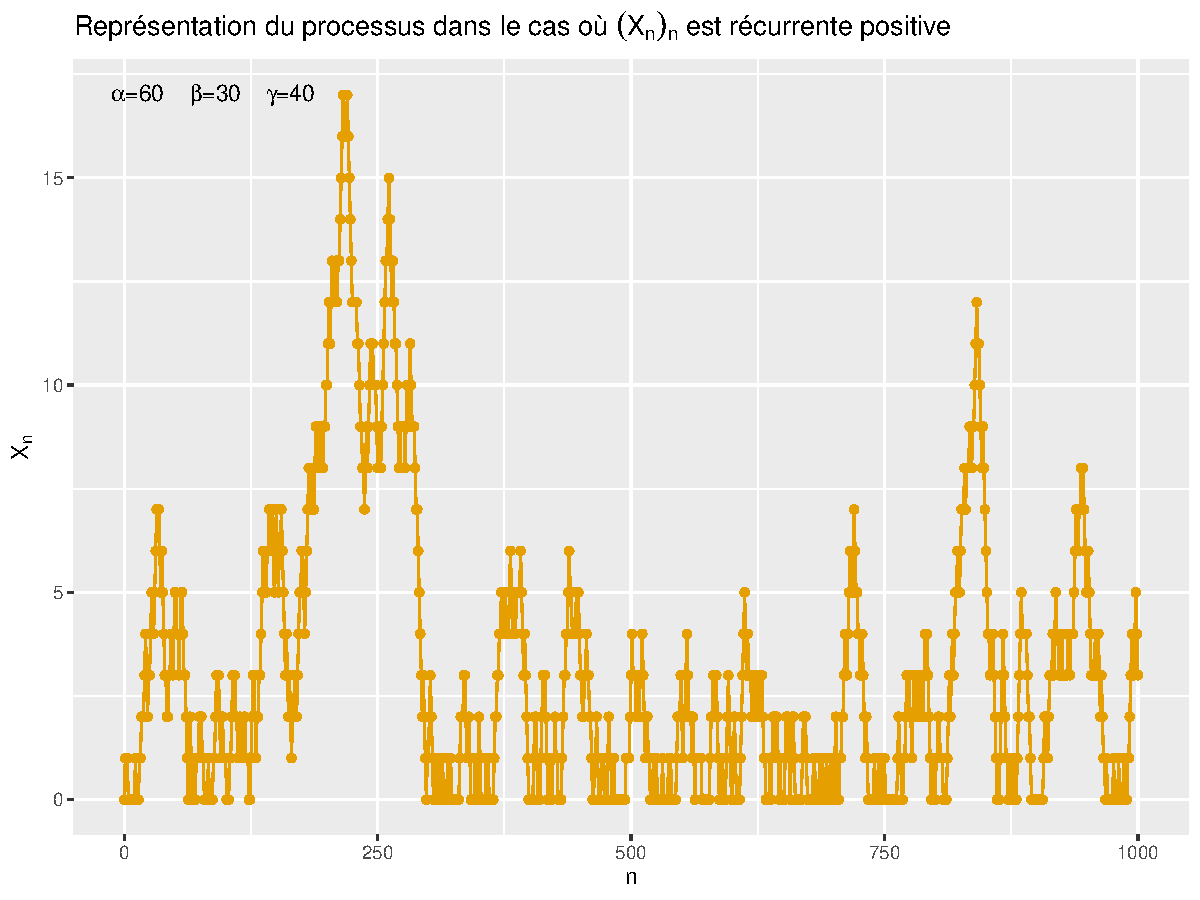
\includegraphics[scale=0.45]{RecPos60_30_40.pdf}
    \end{minipage}
    \hfill%
    \vspace{0.1cm}
    \begin{minipage}[c]{0.50\linewidth}
        \centering
        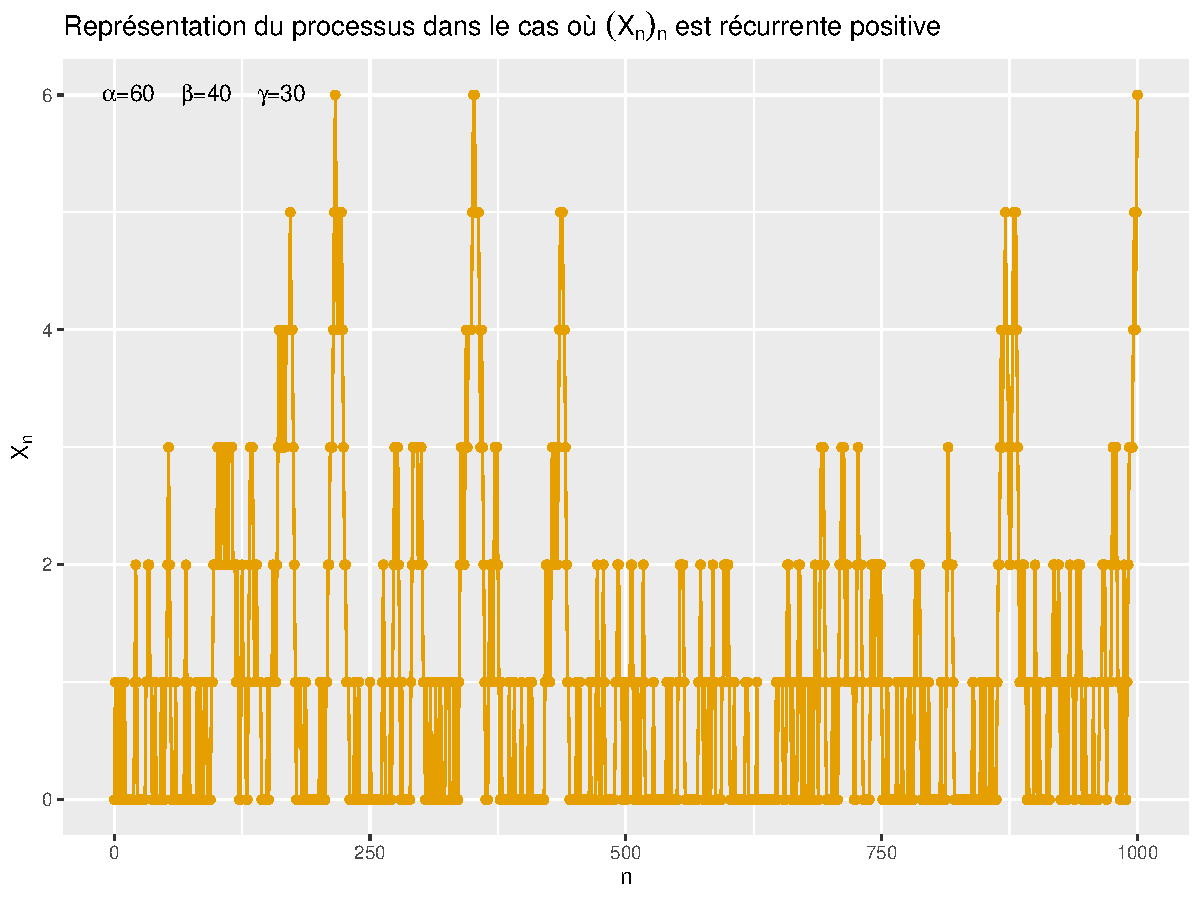
\includegraphics[scale=0.45]{RecPos60_40_30.pdf}  
    \end{minipage}
    \caption{Représentation du processus dans le cas récurrent positif}
    \label{fig_rec_positif}
\end{figure}

\begin{figure}[h!]
    \begin{minipage}[c]{0.25\linewidth}
        \centering
        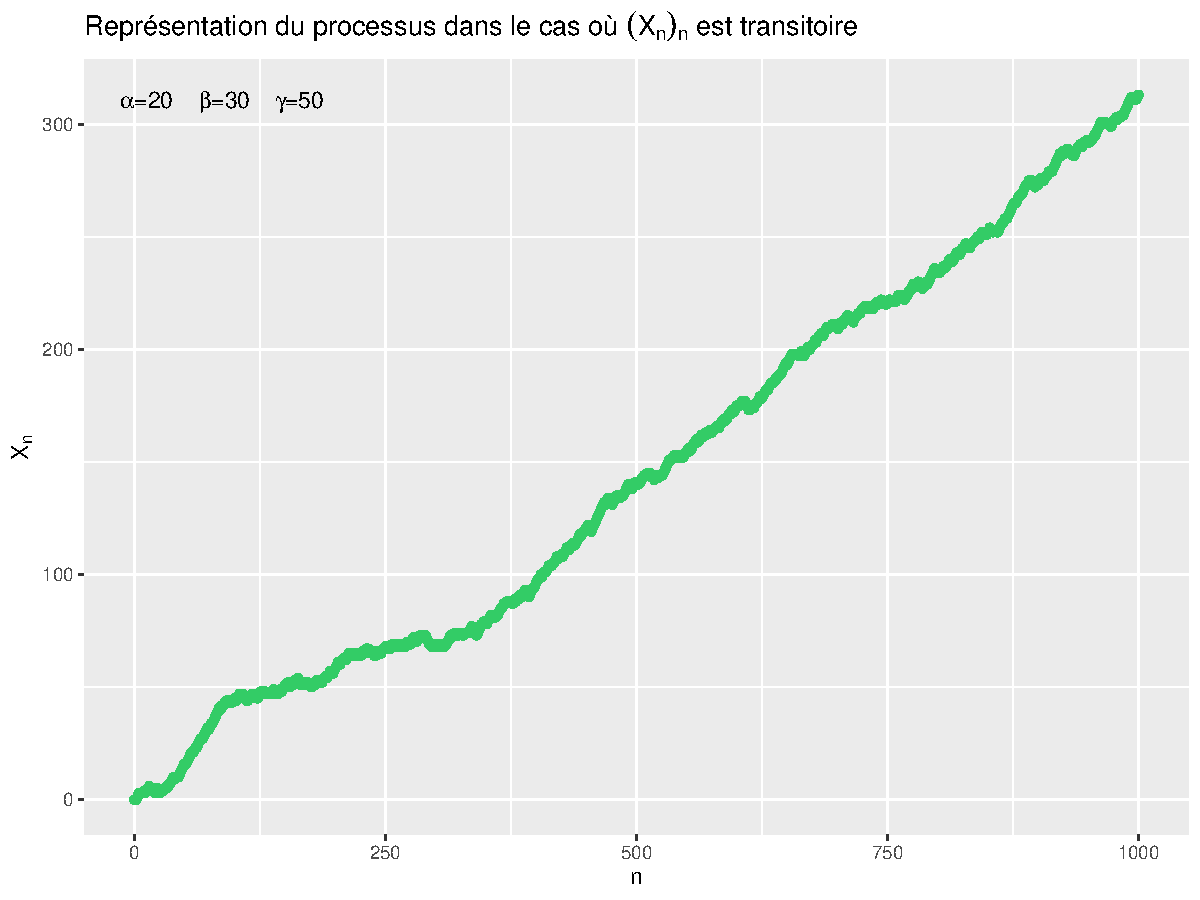
\includegraphics[scale=0.45]{Transi20_30_50.pdf}
    \end{minipage}
    \hfill%
    \vspace{0.1cm}
    \begin{minipage}[c]{0.50\linewidth}
        \centering
        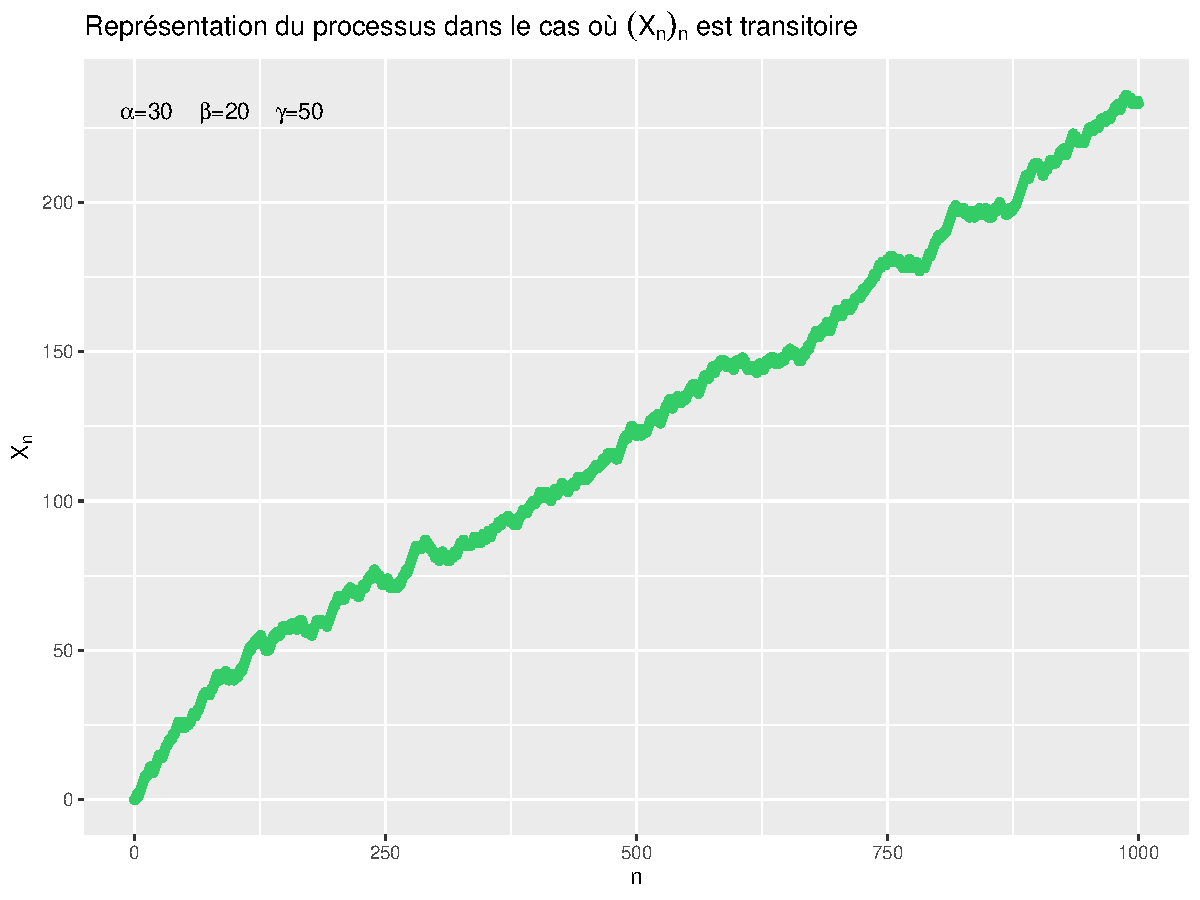
\includegraphics[scale=0.45]{Transi30_20_50.pdf}
    \end{minipage}
      \caption{Représentation du processus dans le cas transitoire}
      \label{fig_transitoire}
\end{figure}

\begin{figure}[h!]
    \begin{minipage}[c]{0.25\linewidth}
        \centering
        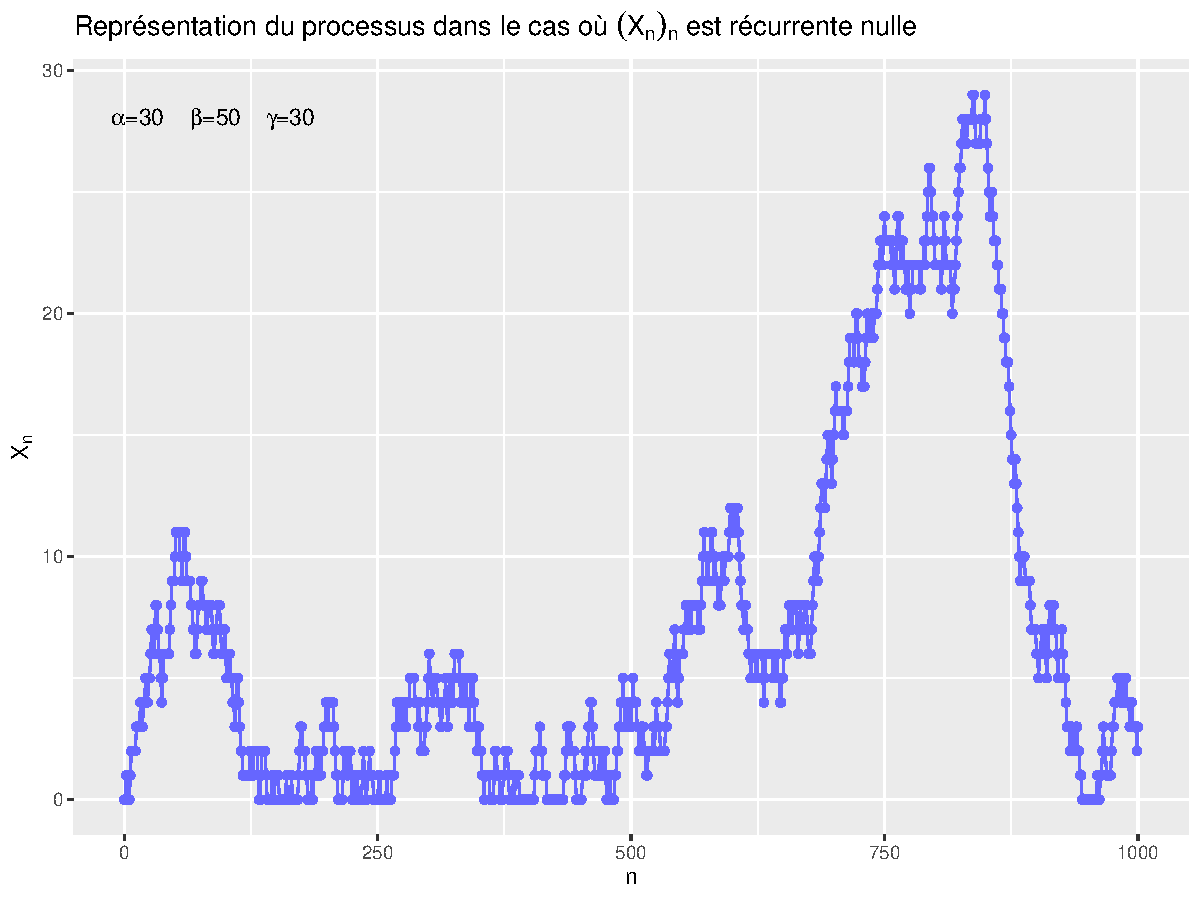
\includegraphics[scale=0.45]{RecNulle30_50_30.pdf}
    \end{minipage}
    \hfill%
    \vspace{0.1cm}
    \begin{minipage}[c]{0.50\linewidth}
        \centering
        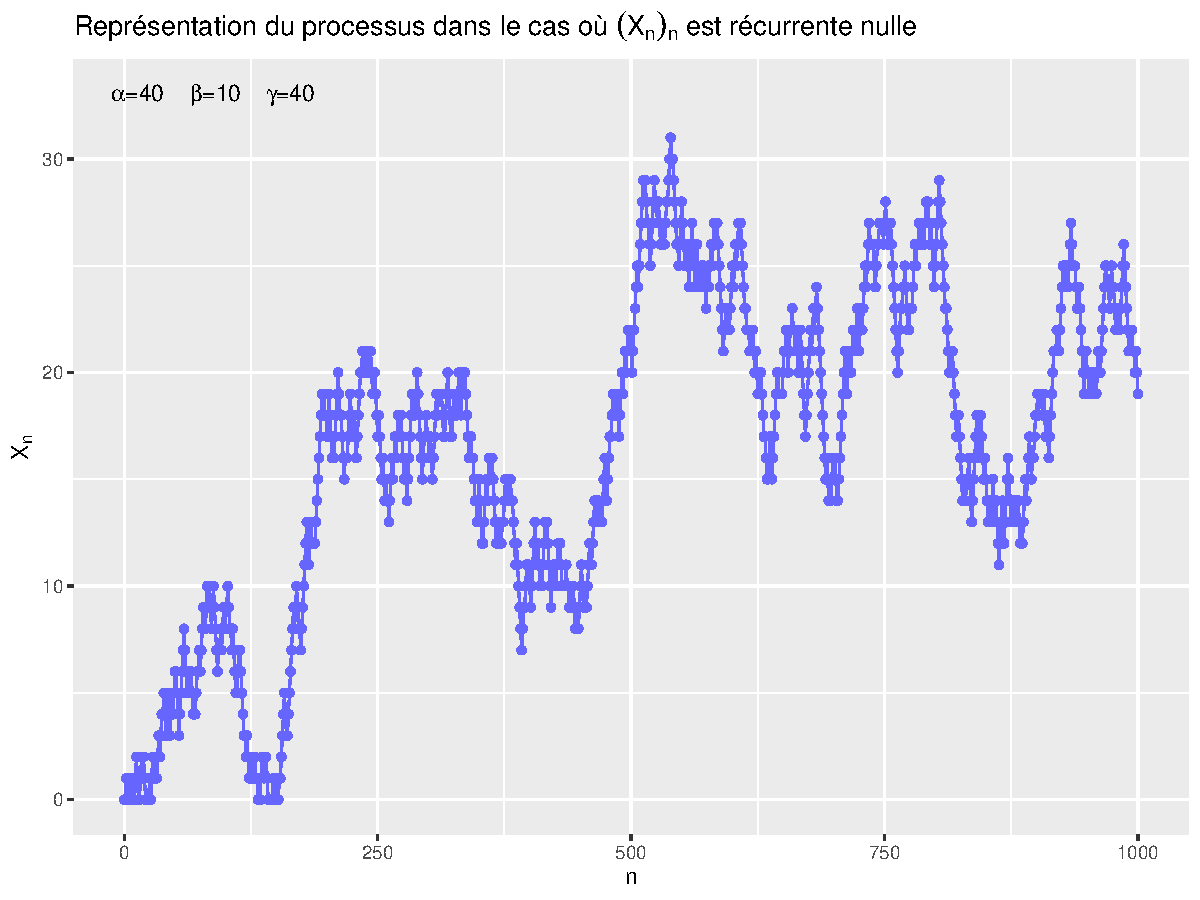
\includegraphics[scale=0.45]{RecNulle40_10_40.pdf}
    \end{minipage}
      \caption{Représentation du processus dans le cas récurrent nul}
      \label{fig_rec_nul}
\end{figure}
 
Tout d'abord, la figure \ref{fig_rec_positif} est composé de deux graphiques, ici en jaune, simulant la chaîne de Markov telle que cette dernière soit récurrente positive, c'est-à-dire que le taux de guérison soit supérieur au taux de contamination. Nous constatons des retours en $0$ très fréquents, c'est-à-dire qu'en temps long, l'épidémie est contrôlée. \\
\\
Par la suite, dans la figure \ref{fig_transitoire}, nous avons simulé en vert les deux graphiques représentant la chaîne de Markov dans le cas transitoire, c'est-à-dire lorsque le taux de guérison est inférieur au taux de contamination. Sur ces graphiques, nous pouvons voir qu'il n'y a pratiquement pas de retour en $0$. Le nombre de contaminés augmente dans le temps avec de légère fluctuation. De ce fait, l'épidémie n'est pas contrôlée : le nombre de contaminés tend vers $+\infty$.\\
\\
Pour finir, les deux derniers graphiques de la figure \ref{fig_rec_nul} simulent la chaîne de Markov dans le cas récurrent nul, c'est-à-dire que le taux de guérison est égal au taux de contamination. Sur ces graphiques, nous observons des retours en $0$ moins récurrent que dans les graphiques de la figure \ref{fig_rec_positif}. Le nombre de contaminés n'explose pas comme dans le cas transitoire mais reste tout de même élevé.
\\
\\
\\
\\
Finalement, ce modèle d'épidémie simple nous a permis d'avoir une première approche du comportement de l'épidémie en temps long selon les valeurs des taux de guérison et contamination. Un taux de guérison supérieur ou égal au taux de contamination engendrera de fortes fluctuations et permettra d'éviter une explosion du nombre de malades. Dans le cas contraire, ce nombre augmentera considérablement sur la durée avec de légères variations, avec une probabilité de retour en $0$ de plus en plus faible. Cependant, vu que l'évolution d'une épidémie dépend du nombre de contaminés $X_n = i$, ce modèle avec des probabilités constantes par rapport à $i$ n'est pas très proche de la réalité. Nous allons donc dans le prochain chapitre définir des nouveaux modèles plus adaptés et étudier leurs caractéristiques.

\chapter{Modèles d'épidémies complexifiés}


L'objectif de ce chapitre est de mettre en place deux modèles complexifiés où la probabilité de $X_{n+1} = j$ sachant que $X_n = i$ dépend de l'état $i$. Nous étudierons dans un premier temps le modèle où les guérisons ont plus d'impact que les contaminations. Nous analyserons ensuite le modèle contraire dans un second temps.

\section{Modèle de guérison}
\subsection{Construction du modèle}
\vspace{0.6cm}

Nous allons construire un modèle qui renforce la probabilité de guérison en fonction du nombre de personnes atteintes par la maladie. Ce modèle est basé sur le modèle précédent où les probabilités de contamination, guérison et stagnation ont été modifiées. Nous avons alors la définition suivante.
\\
\begin{definition}
On définit $(X_n)_{n\geq0}$ le processus où pour $n$ fixé, $X_n$  représente le nombre d'individus infectés par la maladie à l'instant $n$. Nous choisissons une échelle de temps assez petite par rapport à la dynamique de l'épidémie, pour que le passage de $n$ à $n+1$ correspondent à au plus une personne contaminée ou guérie en plus. 
\\
\\
Soit $(\alpha, \beta, \gamma) \in (\mathbb{R}_+^*)^3$. Il y a donc trois possibilités conditionnellement à $X_n = i, \, \, \forall i \in \mathbb{N}^*$ :  
\\
\begin{itemize}
\item une guérison avec une probabilité $\alpha_i=\frac{i \times \alpha}{i \times \alpha+\beta+\gamma}.$
\item une inaction avec une probabilité $\beta_i=\frac{\beta}{i \times \alpha+\beta+\gamma}.$
\item une contamination avec une probabilité $\gamma_i=\frac{\gamma}{i \times \alpha+\beta+\gamma}.$
\end{itemize}
\vspace{0.5cm}
Pour $i=0$, il ne peut pas y avoir de guérison puisqu'il n'y a aucune personne infectée. Nous avons alors :
\\
\begin{itemize}
\item une inaction avec une probabilité $\beta_0 = \frac{\beta}{\beta+\gamma}.$
\item une contamination avec une probabilité $\gamma_0=\frac{\gamma}{\beta+\gamma}.$
\end{itemize}
\vspace{0.5cm}

Chaque individu supplémentaire accentue donc le taux de guérison. Nous supposons que $X_{0} = 0$ et nous avons donc :
\\
\begin{itemize}
\item $\forall n \in \mathbb{N}$, \, si $X_n=0$,\, alors $X_{n+1} = \left\{
    \begin{array}{ll}
        X_n+1 & \mbox{si le (n+1)ème événement est une contamination } \\
        X_n & \mbox{sinon. }
    \end{array}
\right. $
\item $\forall n \in \mathbb{N}^*$, \, si $X_n > 0$,\, alors $X_{n+1} = \left\{
    \begin{array}{ll}
        X_n+1 & \mbox{si le (n+1)ème événement est une contamination} \\
        X_n-1 & \mbox{si le (n+1)ème événement est une guérison} \\
        X_n & \mbox{sinon. }\\
    \end{array}
\right. $
\end{itemize}
\end{definition}
\begin{prop}
Le processus $(X_n)_{n \in \mathbb{N}}$ est une chaîne de Markov de loi initiale $\delta_0$ et de matrice de transition :
$$P=
\begin{pmatrix}
        \beta_0 & \gamma_0 & 0 & 0 & \cdots \\ 
         \alpha_1 & \beta_1 & \gamma_1 & 0 & \cdots\\
         0 & \alpha_2 & \beta_2 & \gamma_2 & \cdots\\
        \vdots &\ddots & \ddots & \ddots & \ddots \\ 
\end{pmatrix}$$
\end{prop}
\begin{proof}
La preuve est la même que celle de la proposition \ref{simple_markov} en prenant cette fois $(U_n)_{n\in \mathbb{N}}$ une suite de variables aléatoires indépendantes à valeurs dans $\{-1, 0, 1\}$ telles que $\forall n \in \mathbb{N}$: \\
\begin{itemize}
    \item $\mathbb{P}(U_n=1)= \frac{\gamma}{i \times \alpha+\beta+\gamma},$
    \item $\mathbb{P}(U_n=0)= \frac{\beta}{i \times \alpha+\beta+\gamma},$
    \item $\mathbb{P}(U_n=-1)= \frac{i \times \alpha}{i \times \alpha+\beta+\gamma}.$
\end{itemize}
\end{proof}

\begin{figure}[h!]
    \centering
    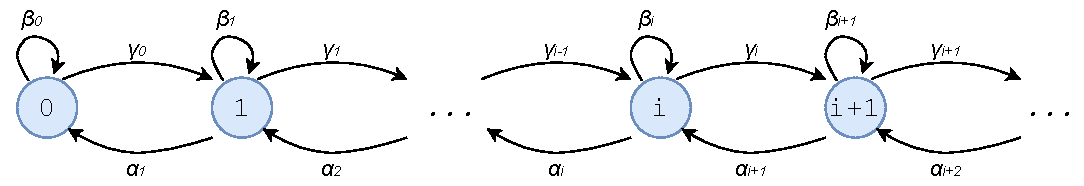
\includegraphics[scale=1]{graphe_model_complexe1.pdf} 
   \caption{Graphe orienté du modèle de guérison}
    \label{fig:graph}
\end{figure}

Nous obtenons alors le graphe associé, représenté dans la figure \ref{fig:graph}. Nous pouvons constater sur la graphe qu'il y a une fois de plus une seule classe, et donc que la chaîne est irréductible. Nous avons également la proposition suivante.
\begin{prop}\label{aperiodique_guerison}
La chaîne $(X_n)_{n \in \mathbb{N}}$ est apériodique.
\end{prop}
\begin{proof}
La preuve est similaire à celle de la proposition \ref{aperiodique}.
\end{proof}

\subsection{Évaluation de la propagation de l'épidémie}
\vspace{0.6cm}

Nous souhaitons dans cette section étudier la nature de notre processus. Nous allons calculer la probabilité d'atteindre $0$ infecté avec ces nouveaux paramètres. Pour cela, nous avons le théorème suivant.

\begin{thm}
La chaîne de Markov $(X_n)_{n \in \mathbb{N}}$ est récurrente.
\end{thm}
\begin{proof}
Soit $T_0$ le temps d'atteinte en $0$. Nous cherchons à calculer $\forall i\in \mathbb{N}, \ \mathbb{P}_i(T_0 < \infty)$. Soit i$\in\mathbb{N}$. On pose $u_i=\mathbb{P}_i(T_0 < \infty)$ et $u=(u_i,\  i\in \mathbb{N})$. Alors par le théorème \ref{th2}, $u$ est la plus petite solution  positive du système : 

\begin{align*}
(S) : \left\{
\begin{array}{ll}
        u_0=1\\
        u_i= \sum\limits_{j\in E} p_{ij}u_j \ \ \ \forall i \in \mathbb{N}^*
    \end{array}
\right.
&\Longleftrightarrow  \left\{
\begin{array}{ll}
        u_0=1\\
        u_i= \alpha_i u_{i-1} + \beta_i u_i + \gamma_i u_{i+1} \ \ \ \forall i \in \mathbb{N}^*
    \end{array}
\right.  \\
&\Longleftrightarrow \left\{
\begin{array}{ll}
        u_0=1\\
        \alpha_i u_{i-1} + (\beta_i-1) u_i + \gamma_i u_{i+1} = 0 \ \ \ \forall i \in \mathbb{N}^*
    \end{array}
\right.  \\
 &\Longleftrightarrow \left\{
\begin{array}{ll}
        u_0=1\\
        \alpha_i u_{i-1} - (\alpha_i+\gamma_i) u_i + \gamma_i u_{i+1} = 0 \ \ \ \forall i \in \mathbb{N}^*
    \end{array}
\right.  \\
 &\Longleftrightarrow \left\{
\begin{array}{ll}
        u_0=1\\
        i \, \alpha \, u_{i-1} - (i \, \alpha+\gamma) u_i + \gamma u_{i+1} = 0 \ \ \ \forall i \in \mathbb{N}^*.
    \end{array}
\right. 
\end{align*}

Montrons par double récurrence que $\forall i \geqslant 2$:
$$u_i = u_1 + (u_1 - 1)\left(\frac{\alpha}{\gamma}\right)^{i-1} \sum_{j=1}^{i-1}(i-j)!\left(\frac{\gamma}{\alpha}\right)^{j-1}.$$

\textbf{Initialisation}: pour $i=2$ et $i=3$, nous avons :
\begin{align*}
\gamma u_2 = -\alpha u_0 + (\alpha + \gamma) u_1 &\iff \gamma u_2 = - \alpha + (\alpha + \gamma)u_1 \\
&\iff u_2 = - \frac{\alpha}{\gamma} + \frac{\alpha + \gamma}{\gamma} u_1 \\
&\iff u_2 = \frac{\alpha}{\gamma}(u_1 - 1) + u_1.
\end{align*}
La relation est vraie pour $i=2$.
\begin{align*}
\gamma u_3 = -2 \alpha u_1 + (2 \alpha + \gamma) u_2 &\iff u_3 = -2 \left(\frac{\alpha}{\gamma}\right) u_1 + (2 \alpha + \gamma)\left(\frac{-\alpha + (\alpha + \gamma) u_1}{\gamma^2}\right) \\
&\iff u_3 = \frac{-2 \alpha^2 + 2 \alpha^2 u_1 + 2 \alpha \gamma u_1 - \alpha \gamma + \alpha \gamma u_1 + \gamma^2 u_1 -2 \alpha \gamma u_1}{\gamma^2} \\
&\iff u_3 = u_1 \left(\frac{-2 \alpha^2 + \alpha \gamma + \gamma^2}{\gamma^2}\right) + \frac{-2 \alpha^2 - \alpha \gamma}{\gamma^2} \\
&\iff u_3 = u_1 \left(\frac{\alpha}{\gamma}\right)^{2} \sum_{j=1}^{3}(i-j)!\left(\frac{\gamma}{\alpha}\right)^{j-1} - \left(\frac{\alpha}{\gamma}\right)^{2} \sum_{j=1}^{2}(i-j)!\left(\frac{\gamma}{\alpha}\right)^{j-1} \\
&\iff u_3 = (u_1 - 1)\left(\frac{\alpha}{\gamma}\right)^{2} \sum_{j=1}^{2}(i-j)!\left(\frac{\gamma}{\alpha}\right)^{j-1} + u_1.
\end{align*}
La relation est vraie pour $i=3$.\\

\textbf{Hérédité}: supposons la propriété vraie aux ordres $i$ et $i+1$. Montrons-là à l'ordre $i+2$.\\

Nous avons les hypothèses de récurrence suivantes : 
$$u_i = u_1 + (u_1 - 1)\left(\frac{\alpha}{\gamma}\right)^{i-1} \sum_{j=1}^{i-1}(i-j)!\left(\frac{\gamma}{\alpha}\right)^{j-1}.$$
$$u_{i+1} = u_1 + (u_1 - 1)\left(\frac{\alpha}{\gamma}\right)^{i} \sum_{j=1}^{i}(i+1-j)!\left(\frac{\gamma}{\alpha}\right)^{j-1}
.$$
Nous avons : $\gamma \, u_{i+2} = -(i+1) \alpha u_i + ((i+1) \alpha + \gamma) u_{i+1} \iff u_{i+2} = -(i+1) \left(\frac{\alpha}{\gamma}\right) u_i + \frac{(i+1) \alpha + \gamma}{\gamma} u_{i+1}$.
\\

Nous allons procéder dans la suite de la démonstration avec des changements d'indices du type $k=j+2$ pour la première somme et $k=j+1$ pour la deuxième. Nous obtenons alors :

\begin{align*}
u_{i+2} &= -(i+1) \frac{\alpha}{\gamma} \left(u_1 + (u_1 - 1)\left(\frac{\alpha}{\gamma}\right)^{i-1} \sum_{j=1}^{i-1}(i-j)!\left(\frac{\gamma}{\alpha}\right)^{j-1}\right) \\
&+ \frac{((i+1) \alpha + \gamma)}{\gamma} \left(u_1 + (u_1 - 1)\left(\frac{\alpha}{\gamma}\right)^{i} \sum_{j=1}^{i}(i+1-j)!\left(\frac{\gamma}{\alpha}\right)^{j-1}\right) \\
&= -(i+1) \frac{\alpha}{\gamma} \left(u_1 + (u_1 - 1)\left(\frac{\alpha}{\gamma}\right)^{i-1} \sum_{k=3}^{i+1}(i+2-k)!\left(\frac{\gamma}{\alpha}\right)^{k-3}\right) \\
&+ \frac{((i+1) \alpha + \gamma)}{\gamma} \left(u_1 + (u_1 - 1)\left(\frac{\alpha}{\gamma}\right)^{i} \sum_{k=2}^{i+1}(i+2-k)!\left(\frac{\gamma}{\alpha}\right)^{k-2}\right) \\
&= -(i+1) \frac{\alpha}{\gamma} \left(u_1 + (u_1 - 1)\left(\frac{\alpha}{\gamma}\right)^{i-1} \sum_{k=3}^{i+1}(i+2-k)!\left(\frac{\gamma}{\alpha}\right)^{k-3}\right) \\
&+ \frac{((i+1) \alpha + \gamma)}{\gamma} \left(u_1 + (u_1 - 1)\left(\frac{\alpha}{\gamma}\right)^{i-1} \sum_{k=3}^{i+1}(i+2-k)!\left(\frac{\gamma}{\alpha}\right)^{k-3} + i! \left(\frac{\alpha}{\gamma}^i(u_1 - 1\right)\right) \\
&= -\frac{(i+1)\alpha}{\gamma} u_1 + \frac{(i+1)\alpha}{\gamma} u_1 + \frac{(i+1)\alpha}{\gamma} i! \left(\frac{\alpha}{\gamma}\right)^i (u_1 - 1) + \left(\frac{\alpha}{\gamma}\right)^{i-1} \sum_{k=3}^{i+1}(i+2-k)!\left(\frac{\gamma}{\alpha}\right)^{k-3} \\
&+ i! \left(\frac{\alpha}{\gamma}\right)^i (u_1 - 1) + u_1 \\
&= (i+1)! \left(\frac{\alpha}{\gamma}\right)^{i+1} (u_1 - 1) + \sum_{k=3}^{i+1}(i+2-k)!\left(\frac{\gamma}{\alpha}\right)^{k-1} \left(\frac{\alpha}{\gamma}\right)^{i+1} + i! \left(\frac{\alpha}{\gamma}\right)^i (u_1 - 1) + u_1 \\
&= \left(\frac{\alpha}{\gamma}\right)^{i+1} (u_1 - 1) \left((i+1)! + i! \frac{\gamma}{\alpha} + \sum_{k=3}^{i+1}(i+2-k)!\left(\frac{\gamma}{\alpha}\right)^{k-1} \right) + u_1 \\
&= \left(\frac{\alpha}{\gamma}\right)^{i+1} (u_1 - 1) \left(\sum_{k=1}^{i+1}(i+2-k)!\left(\frac{\gamma}{\alpha}\right)^{k-1} \right) + u_1.
\end{align*}
La relation est vraie au rang $i+2$. Ainsi, la double récurrence est établie et nous avons finalement $\forall i \geqslant 2$:
$$u_i = u_1 + (u_1 - 1)\left(\frac{\alpha}{\gamma}\right)^{i-1} \sum_{j=1}^{i-1}(i-j)!\left(\frac{\gamma}{\alpha}\right)^{j-1}.$$

Or, d'après le théorème \ref{th2}, $(u_i, i \in E)$ est la plus petite solution positive du système. Nous avons alors $\forall i \in E$:
\begin{align*}
u_i \geqslant 0 &\iff  u_1 + (u_1 - 1)\left(\frac{\alpha}{\gamma}\right)^{i-1} \sum_{j=1}^{i-1}(i-j)!\left(\frac{\gamma}{\alpha}\right)^{j-1} \geqslant 0 \\
&\iff u_1 \left(1 + \left(\frac{\alpha}{\gamma}\right)^{i-1} \sum_{j=1}^{i-1}(i-j)!(\frac{\gamma}{\alpha})^{j-1}\right) \geqslant  \left(\frac{\alpha}{\gamma}\right)^{i-1}\sum_{j=1}^{i-1}(i-j)!\left(\frac{\gamma}{\alpha}\right)^{j-1} \\
&\iff u_1 \geqslant \frac{ (\frac{\alpha}{\gamma})^{i-1}\sum\limits_{j=1}^{i-1}(i-j)!(\frac{\gamma}{\alpha})^{j-1}}{1 + (\frac{\alpha}{\gamma})^{i-1} \sum\limits_{j=1}^{i-1}(i-j)!(\frac{\gamma}{\alpha})^{j-1}} \\
&\iff u_1 \geqslant \frac{1}{\frac{1}{(\frac{\alpha}{\gamma})^{i-1}\sum\limits_{j=1}^{i-1}(i-j)!(\frac{\gamma}{\alpha})^{j-1}}+1}\\
&\iff u_1 \geqslant \frac{1}{\frac{1}{A_i} + 1} \, \, \, \text{ avec } A_i = \left(\frac{\alpha}{\gamma}\right)^{i-1} \sum_{j=1}^{i-1}(i-j)!\left(\frac{\gamma}{\alpha}\right)^{j-1}.
\end{align*}

En faisant le changement d'indices $k=i-j$, nous avons :
\begin{align*}
A_i &= \left(\frac{\alpha}{\gamma}\right)^{i-1} \sum_{j=1}^{i-1}(i-j)!\left(\frac{\gamma}{\alpha}\right)^{j-1} \\
&= \left(\frac{\alpha}{\gamma}\right)^{i-1} \sum_{k=1}^{i-1}k!\left(\frac{\gamma}{\alpha}\right)^{i-k-1} \\
&= \left(\frac{\alpha}{\gamma}\right)^{i-1} \left(\frac{\gamma}{\alpha}\right)^{i-1} \sum_{k=1}^{i-1}k!\left(\frac{\alpha}{\gamma}\right)^k \\
&= \sum_{k=1}^{i-1}k!\left(\frac{\alpha}{\gamma}\right)^k \\
&\geqslant (i-1)! \left(\frac{\alpha}{\gamma}\right)^{i-1}
\end{align*}

Or : $\forall \alpha > 0, \forall \gamma > 0, \, \, \lim\limits_{i \rightarrow +\infty} (i-1)! \left(\frac{\alpha}{\gamma}\right)^{i-1} = +\infty$, d'où : $\lim\limits_{i \rightarrow +\infty} A_i = +\infty$.
\\
\\
Ainsi, par quotient, lorsque $i$ tend vers $+\infty$ , $u_1 \geqslant 1$. Comme $u_1 = \mathbb{P}_{1}(T_0 < \infty) \in [0,1]$, alors $u_1=1$. Nous en déduisons  :
$$\forall i \in E, \, \, u_i = 1.$$

Nous avons donc $\forall \alpha > 0, \, \forall \gamma > 0, \, \forall i \in \mathbb{N}$ :
\begin{align*}
\mathbb{P}_0(S_0 < \infty) &= \sum_{j\in E}{\mathbb{P}_j(T_0 < \infty)p_{0j}} \\
&= \sum_{j\in E}u_j \, {p_{0j}} \\
&= u_0 \beta_0 + u_1 \gamma_0 \\
&= \frac{\beta}{\beta + \gamma} + \frac{\gamma}{\beta + \gamma} \\
&= 1.
\end{align*}

Nous venons de démontrer que l'état $0$ était récurrent, peu importe les paramètres. Vu que $(X_n)_{n \in \mathbb{N}}$ est irréductible, $(X_n)_{n \in \mathbb{N}}$ est ainsi récurrente par propriété de classe.
\end{proof}

\subsection{Récurrence positive}
\vspace{0.6cm}

Maintenant que nous savons que la chaîne est récurrente, nous souhaitons voir dans quels cas elle est récurrente positive ou non. Nous pouvons énoncer le résultat suivant, que nous allons démontrer.

\begin{thm}\label{th_loi_inv}
La chaîne de Markov $(X_n)_{n \in \mathbb{N}}$ est récurrente positive.
\end{thm}
\begin{proof}
Vu que la chaîne est irréductible et récurrente, d'après le théorème \ref{th6}, $(X_n)_{n\in\mathbb{N}}$ admet une unique mesure invariante $\pi=(\pi_i\, , \, i \in E)$ à une constante multiplicative près et $\forall i \in E, \, \, \, 0< \pi_i<\infty$. Calculons :
\begin{align*}
\pi P=\pi
&\iff (\pi_0,\pi_1,...) \begin{pmatrix}
        \beta_0 & \gamma_0 & 0 & 0 & \cdots \\ 
         \alpha_1 & \beta_1 & \gamma_1 & 0 & \cdots\\
         0 & \alpha_2 & \beta_2 & \gamma_2 & \cdots\\
        \vdots &\ddots & \ddots & \ddots & \ddots \\ 
\end{pmatrix} = (\pi_0,\pi_1,...)\\
&\iff 
\left\{
\begin{array}{ll}
        \pi_0=\beta_0\pi_0+\alpha_1\pi_1 \\
        \pi_i=\gamma_{i-1}\pi_{i-1}+\beta_{i}\pi_{i}+\alpha_{i+1}\pi_{i+1} \, \, \, \forall i \in \mathbb{N}^*
    \end{array}
\right. \\
&\iff \left\{
\begin{array}{ll}
        (\beta_0-1)\pi_0+\alpha_1\pi_1 = 0 \\
        \gamma_{i-1}\pi_{i-1}+(\beta_{i}-1)\pi_{i}+\alpha_{i+1}\pi_{i+1} = 0 \, \, \, \forall i \in \mathbb{N}^*
    \end{array}
\right. \\
&\iff \left\{
\begin{array}{ll}
         -\gamma_0\pi_0+\alpha_1\pi_1 = 0\\
        \gamma_{i-1}\pi_{i-1}-(\alpha_i + \gamma_i)\pi_{i}+\alpha_{i+1}\pi_{i+1} = 0 \, \, \, \forall i \in \mathbb{N}^*
    \end{array}
\right. \\ 
&\iff \left\{
\begin{array}{ll}
       -\gamma\pi_0+\alpha\pi_1 = 0\\
        \gamma\pi_{i-1}-(i\alpha + \gamma)\pi_{i}+\alpha(i+1)\pi_{i+1} = 0 \, \, \, \forall i \in \mathbb{N}^*.
    \end{array}
\right.
\end{align*}
\\
Montrons par double récurrence que $\forall i \geqslant 1$:
$$\pi_i = \left(\frac{\gamma}{\alpha}\right)^{i}\frac{\pi_0}{i!}.$$

\textbf{Initialisation}: Pour $i=1$, nous avons :
\begin{align*}
 -\gamma\pi_0+\alpha\pi_1 = 0 \iff  \frac{\gamma}{\alpha}\pi_0=\pi_1.
\end{align*}
La relation est vraie pour $i=1$.\\

Pour $i=2$, nous avons :
\begin{align*}
 \gamma\pi_{0}-(\alpha + \gamma)\pi_{1}+2\alpha\pi_{2} = 0 &\iff 2\alpha\pi_{2}=(\alpha + \gamma)\pi_{1}- \gamma\pi_{0} \iff 2\alpha\pi_{2}=(\alpha + \gamma)\frac{\gamma}{\alpha}\pi_0- \gamma\pi_{0}\\
 &\iff  2\alpha\pi_{2}=\pi_0((\alpha + \gamma)\frac{\gamma}{\alpha}- \gamma ) \iff 2\alpha\pi_{2}=\pi_0\frac{\gamma^2}{\alpha} \\
 &\iff \pi_{2}=\frac{\pi_0}{2}\left(\frac{\gamma}{\alpha}\right)^2.
\end{align*}
La relation est vraie pour $i=2$.\\

\textbf{Hérédité}: supposons la propriété vraie aux ordres $i-1$ et $i$. Montrons-là à l'ordre $i+1$.\\

Nous avons les hypothèses de récurrence suivantes : 
$$\pi_{i-1} = \left(\frac{\gamma}{\alpha}\right)^{i-1}\frac{\pi_0}{(i-1)!} \, \, \, \text{ et } \, \, \, \pi_i = \left(\frac{\gamma}{\alpha}\right)^{i}\frac{\pi_0}{i!}.$$

Nous avons : 
\begin{align*}
 \gamma\pi_{i-1}-(i\alpha + \gamma)\pi_{i}+(i+1) \, \alpha \, \pi_{i+1} = 0
 &\iff  (i+1) \, \alpha \, \pi_{i+1}=(i\alpha + \gamma)\pi_{i}- \gamma\pi_{i-1} \\
 &\iff  (i+1) \, \alpha \, \pi_{i+1}=(i\alpha + \gamma)\left(\frac{\gamma}{\alpha}\right)^{i}\frac{\pi_0}{i!}- \gamma\left(\frac{\gamma}{\alpha}\right)^{i-1}\frac{\pi_0}{(i-1)!}\\
&\iff (i+1) \, \alpha \, \pi_{i+1}=\pi_0\frac{\gamma^{i+1}}{i! \, \alpha^{i}}  \\
&\iff \pi_{i+1}=\pi_0\frac{\gamma^{i+1}}{(i+1)! \, \alpha^{i+1}}.
\end{align*}
 
La relation est vraie au rang $i+1$. Ainsi, la double récurrence est établie et nous avons finalement $\forall i \geqslant 1$:
$$\pi_i = \left(\frac{\gamma}{\alpha}\right)^{i}\frac{\pi_0}{i!}.$$

Finalement : $\pi = c_i \left(1, \frac{\gamma}{\alpha}, \frac{\gamma^2}{2 \alpha^2},...,\frac{\gamma^i}{i! \,  \alpha^i},... \right) \text{ avec } c_i \in \mathbb{R}_+^{*}.$ \\

La constante $c_i$ est telle que $\pi_i^i = 1$. Nous avons donc, $\forall i \in \mathbb{N}, \, c_i = \frac{i! \, \alpha^i}{\gamma^i}$. Nous en déduisons :
$$\forall i \in \mathbb{N}, \, \, \mathbb{E}_i[S_i] = \sum\limits_{j=0}^{+\infty} \pi_j^i =  c_i \sum\limits_{j=0}^{+\infty} \left(\frac{\gamma}{\alpha}\right)^j \frac{1}{j!} = c_i \, e^{\frac{\gamma}{\alpha}} < +\infty.$$

Ainsi, $(X_n)_{n \in \mathbb{N}}$ est récurrente positive.
\end{proof}

Nous obtenons donc que la chaîne est récurrente positive, peu importe les valeurs des taux de guérison et contamination. La preuve du théorème \ref{th_loi_inv} nous donne plusieurs résultats intéressants.

\begin{prop}
La mesure $\pi$ est l'unique loi invariante de $(X_n)_{n \in \mathbb{N}}$ et nous avons : $$\forall i \in \mathbb{N}, \, \, \pi_i = \frac{\gamma^i \, e^{-\frac{\gamma}{\alpha}}}{i! \, \alpha^i}.$$ 
\end{prop}
\begin{proof}
La chaîne $(X_n)_{n \in \mathbb{N}}$ est récurrente positive et $\pi$ vérifie $\pi P = \pi$. Alors, d'après le théorème \ref{th61}, $\pi$ est l'unique loi invariante de $(X_n)_{n \in \mathbb{N}}$. D'après la preuve du théorème \ref{th_loi_inv}, nous avons $\forall i \in \mathbb{N}$ :
$$\pi_i = \frac{1}{\mathbb{E}_i[S_i]} = \frac{1}{c_i \, e^{\frac{\gamma}{\alpha}}} = \frac{\gamma^i \, e^{-\frac{\gamma}{\alpha}}}{i! \, \alpha^i}.$$
\end{proof}
\begin{remark}
Nous avons en particulier : $\mathbb{E}_0[S_0] = c_0 \, e^{\frac{\gamma}{\alpha}} = e^{\frac{\gamma}{\alpha}}.$ Nous constatons que, partant de $0$, le temps de retour espéré en $0$ augmente si le taux de contamination augmente  et diminue si le taux de guérison augmente, ce qui est cohérent.
\end{remark}
\begin{prop}
Nous avons les résultats suivants :
\begin{itemize}
    \item $\forall (i,j) \in \mathbb{N}^2, \, \, \lim\limits_{n \to +\infty} \mathbb{P}_i(X_n = j) = \frac{\gamma^j \, e^{-\frac{\gamma}{\alpha}}}{j! \, \alpha^j}.$
    \item En particulier : $\lim\limits_{n \to +\infty} \mathbb{P}_i(X_n = 0) = e^{-\frac{\gamma}{\alpha}}.$
\end{itemize}
\end{prop}
\begin{proof}
D'après la proposition \ref{aperiodique_guerison}, la chaîne $(X_n)_{n \in \mathbb{N}}$ est apériodique. Vu qu'elle est aussi irréductible et récurrente positive de probabilité invariante $\pi$, alors par le théorème \ref{th3}, $\forall (i,j) \in \mathbb{N}^2$ :
$$\lim\limits_{n \to +\infty} \mathbb{P}_i(X_n = j) = \pi_j = \frac{\gamma^j \, e^{-\frac{\gamma}{\alpha}}}{j! \, \alpha^j}.$$

Ainsi, la probabilité partant de n’importe quel état $j$ différent de $0$ d’atteindre $0$ à long terme est $\frac{\gamma^j \, e^{-\frac{\gamma}{\alpha}}}{j! \, \alpha^j}$. En particulier :
$$\lim\limits_{n \to +\infty} \mathbb{P}_i(X_n = 0) = \pi_0 = e^{-\frac{\gamma}{\alpha}}.$$\\
\end{proof}

\subsection{Ergodicité}
\vspace{0.6cm}

Nous terminons l'étude de ce second modèle de la même manière que le premier, c'est-à-dire en calculant le nombre d’infectés moyen à long terme : $\lim\limits_{n \to +\infty} \frac{1}{n} \sum\limits_{k=0}^{n-1} X_k.$
\begin{thm}
Le nombre d’infectés moyen à long terme du modèle de guérison est : $$\lim\limits_{n \to +\infty} \frac{1}{n} \sum\limits_{k=0}^{n-1} X_k =  \frac{\gamma}{\alpha} \left(1 - e^{-\frac{\gamma}{\alpha}}\right).$$
\end{thm}
\begin{proof}
Soit $f : \mathbb{N} \longrightarrow \mathbb{N}$ la fonction identité, i.e $\forall i \in \mathbb{N}, \, \, f(i) = i.$ Nous avons :
\begin{align*}
\sum_{i=0}^{+\infty} |f(i)| \pi_i &= \sum_{i=0}^{+\infty} i \left(\frac{\gamma}{\alpha}\right)^i \frac{e^{-\frac{\gamma}{\alpha}}}{i!} \\
&= e^{-\frac{\gamma}{\alpha}} \sum_{i=0}^{+\infty} \left(\frac{\gamma}{\alpha}\right)^i \frac{1}{(i-1)!} \\
&=  e^{-\frac{\gamma}{\alpha}} \left(\frac{\gamma}{\alpha}\right)  \sum_{j=1}^{+\infty} \left(\frac{\gamma}{\alpha}\right)^j \frac{1}{(j)!} \\
&= e^{-\frac{\gamma}{\alpha}} \left(\frac{\gamma}{\alpha}\right) \left(e^{\frac{\gamma}{\alpha}}
 - 1 \right) \\
&= \frac{\gamma}{\alpha} - \frac{\gamma}{\alpha} e^{-\frac{\gamma}{\alpha}} \\
&= \frac{\gamma}{\alpha} \left(1 - e^{-\frac{\gamma}{\alpha}}\right) < +\infty.
\end{align*}

Donc : $f$ est $\pi$-intégrable.\\

$(X_n)_{n \in \mathbb{N}}$ est une chaîne de Markov irréductible et récurrente positive de loi invariante $\pi$ et $f$ est $\pi$-intégrable. Alors, d’après le théorème ergodique, pour toute loi initiale $\mu$ :
$$\lim\limits_{n \to +\infty} \frac{1}{n} \sum\limits_{k=0}^{n-1} X_k= \pi f = \sum\limits_{i\in\mathbb{N}} f(i)\pi_i=  \frac{\gamma}{\alpha} \left(1 - e^{-\frac{\gamma}{\alpha}}\right) \text{   }\, \, \, \mathbb{P}_{\mu}-p.s.$$

A long terme, le nombre moyen d'infectés est égal à $ \frac{\gamma}{\alpha} \left(1 - e^{-\frac{\gamma}{\alpha}}\right)$.
\end{proof}

\subsection{Simulations}
\vspace{0.6cm}

Nous allons dans cette section simuler le comportement de notre chaîne de Markov en fonction des différents taux $\alpha, \beta$ et $ \gamma$. Nous obtenons les graphiques de l'évolution du processus dans le temps dans la figure \ref{fig_guerison}. Celui de gauche représente le cas où $\alpha < \gamma$. Nous pouvons observer de grandes oscillations avec quelques retours en $0$. Globalement, le nombre de contaminés ne tend pas vers $+\infty$ et l'épidémie ne se propagera pas à une grande échelle, même en ayant un taux de contamination plus élevé que celui de guérison. Dans le cas où $\alpha > \gamma$ (graphique de droite), les retours en $0$ sont beaucoup plus fréquents : l'épidémie restera toujours sous un seuil relativement faible.

\begin{figure}[h]
    \begin{minipage}[c]{0.25\linewidth}
        \centering
        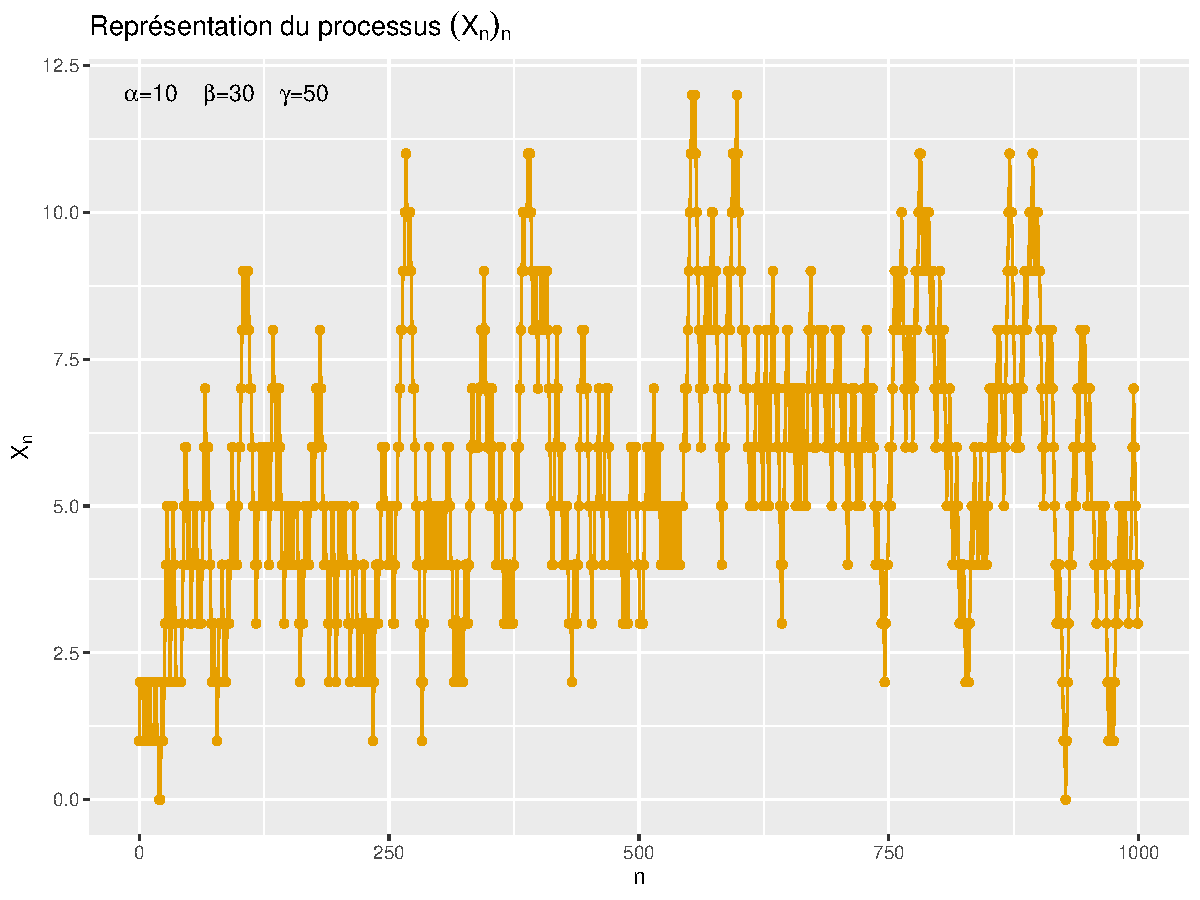
\includegraphics[scale=0.45]{mod1_10_30_50.pdf}
    \end{minipage}
    \hfill%
    \vspace{0.1cm}
    \begin{minipage}[c]{0.50\linewidth}
        \centering
       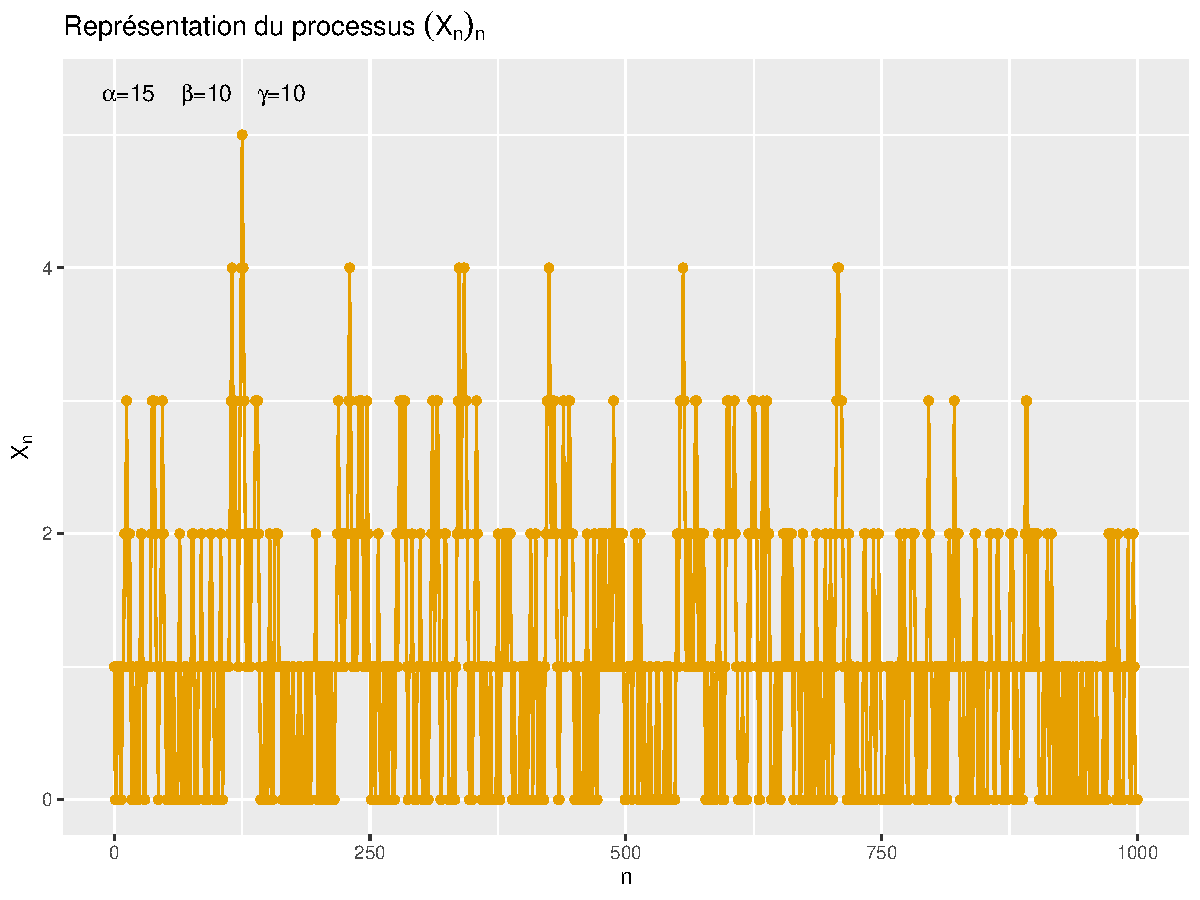
\includegraphics[scale=0.45]{mod1_15_10_10.pdf}
    \end{minipage}
    \caption{Représentation du processus pour le modèle de guérison}
    \label{fig_guerison}
\end{figure}  


\section{Modèle de contamination}

\subsection{Construction du modèle}
\vspace{0.6cm}

Dans ce modèle, nous favorisons cette fois la probabilité d'être contaminé par la maladie. Nous commençons par construire le modèle à l'aide de la définition suivante.
\\
\begin{definition}
On définit $(X_n)_{n\geq0}$ le processus où pour $n$ fixé, $X_n$  représente le nombre d'individus infectés par la maladie à l'instant $n$. Nous choisissons une échelle de temps assez petite par rapport à la dynamique de l'épidémie, pour que le passage de $n$ à $n+1$ correspondent à au plus une personne contaminée ou guérie en plus. 
\\
\\
Soit $(\alpha, \beta, \gamma) \in (\mathbb{R}_+^*)^3$. Il y a donc trois possibilités conditionnellement à $X_n = i, \, \, \forall i \in \mathbb{N}^*$ :  
\\
\begin{itemize}
\item une guérison avec une probabilité $\alpha_i=\frac{\alpha}{\alpha+\beta+i \times \gamma}.$
\item une inaction avec une probabilité $\beta_i=\frac{\beta}{\alpha+\beta+i \times \gamma}.$
\item une contamination avec une probabilité $\gamma_i=\frac{i \times \gamma}{\alpha+\beta+i \times \gamma}.$
\end{itemize}
\vspace{0.5cm}
Pour $i=0$, il ne peut pas y avoir de guérison puisqu'il n'y a aucune personne infectée, et par définition, $\gamma_0 = 0$. Nous avons alors une inaction avec probabilité $1$. De ce fait, nous prenons : $X_0 = 1$. Nous avons alors :
\\
\begin{itemize}
\item $\forall n \in \mathbb{N}$, \, si $X_n=0$,\, alors $X_{n+1} = X_n.$
\item $\forall n \in \mathbb{N}^*$, \, si $X_n > 0$,\, alors $X_{n+1} = \left\{
    \begin{array}{ll}
        X_n+1 & \mbox{si le (n+1)ème événement est une contamination} \\
        X_n-1 & \mbox{si le (n+1)ème événement est une guérison} \\
        X_n & \mbox{sinon. }\\
    \end{array}
\right. $
\end{itemize}
\end{definition}
\begin{prop}
Le processus $(X_n)_{n \in \mathbb{N}}$ est une chaîne de Markov de loi initiale $\delta_0$ et de matrice de transition :
$$P=
\begin{pmatrix}
        1 & 0 & 0 & 0 & \cdots \\ 
         \alpha_1 & \beta_1 & \gamma_1 & 0 & \cdots\\
         0 & \alpha_2 & \beta_2 & \gamma_2 & \cdots\\
        \vdots &\ddots & \ddots & \ddots & \ddots \\ 
\end{pmatrix}$$
\end{prop}
\begin{proof}
La preuve est la même que celle de la proposition \ref{simple_markov} en prenant cette fois $(U_n)_{n\in \mathbb{N}}$ une suite de variables aléatoires indépendantes à valeurs dans $\{-1, 0, 1\}$ telles que $\forall n \in \mathbb{N}$: \\
\begin{itemize}
    \item $\mathbb{P}(U_n=1)= \frac{i \times \gamma}{\alpha+\beta+i \times \gamma},$
    \item $\mathbb{P}(U_n=0)= \frac{\beta}{\alpha+\beta+i \times \gamma},$
    \item $\mathbb{P}(U_n=-1)= \frac{\alpha}{\alpha+\beta+i \times \gamma}.$
\end{itemize}
\end{proof}

La figure \ref{fig:my_label2} représente le graphe orienté associé à la chaîne de Markov et nous permet de visualiser les classes de communication.

\begin{figure}[h]
    \centering
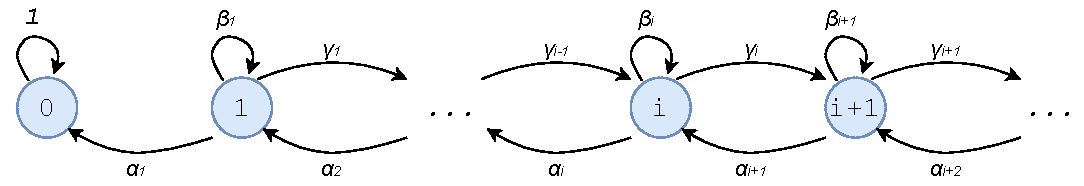
\includegraphics[scale=1]{graphe_model_complexe2.pdf} 
\caption{Graphe orienté du modèle de contamination}
    \label{fig:my_label2}
\end{figure}

\begin{prop}
La chaîne de Markov $(X_n)_{n \in \mathbb{N}}$ est telle que :
\begin{itemize}
    \item elle admet deux classes de communication $C_1=\{0\}$ et $C_2=\mathbb{N}^*.$
    \item $C_1$ est récurrente.
    \item $C_2$ est transitoire.
    \item $0$ est un état absorbant.
\end{itemize}
\end{prop}
\begin{proof}
Nous constatons que l'état $0$ est un état absorbant car $1 \longrightarrow 0$ et $\forall i \in \mathbb{N}^*, \, \, 0 \nrightarrow i$. De plus : $\forall i \in \mathbb{N}^*,\ \  i \longleftrightarrow i+1$. Il y a donc deux classes : $C_1=\{0\}$ et $C_2=\mathbb{N}^*.$
\\
\\
La classe $C_1$ est fermée car $\forall i \in C_2, \, \, 0 \nrightarrow i$. Vu que $C_1$ est finie, alors $C_1$ est récurrente.
\\
\\
La classe $C_2$ est non fermée car $1 \rightarrow 0$ et $0 \notin C_2$. La classe $C_2$ est donc transitoire.
\end{proof}

\subsection{Comportement en temps long}
\vspace{0.6cm}

Le but de cette partie est d'étudier le comportement du processus en temps long. Vu que nous avons deux classes, nous souhaitons savoir la probabilité de sortir de la classe $C_2$ pour pouvoir atteindre $0$ infecté en fonction du nombre de contaminés. Nous avons pour cela le théorème suivant.

\begin{thm}
Soit $T_0$ le temps d'atteinte en $0$. Soit $i \in \mathbb{N}$. On pose $u_i=\mathbb{P}_i(T_0< \infty)$ et $u=(u_i,\  i\in \mathbb{N})$. Alors :
\begin{itemize}
    \item $u_1 = 1 - e^{-\frac{\alpha}{\gamma}}$,
    \item $\lim\limits_{i \rightarrow +\infty} u_i = 0.$
\end{itemize}
\end{thm}
\begin{proof}
D'après le théorème \ref{th2}, $u$ est la plus petite solution positive du système : 

\begin{align*}
(S) : \left\{
\begin{array}{ll}
        u_0=1\\
        u_i= \sum\limits_{j\in \mathbb{N}} p_{ij}u_j \ \ \ \forall i \in \mathbb{N}^*
    \end{array}
\right.
&\Longleftrightarrow  \left\{
\begin{array}{ll}
        u_0=1\\
        u_i= \alpha_i u_{i-1} + \beta_i u_i + \gamma_i u_{i+1} \ \ \ \forall i \in \mathbb{N}^*
    \end{array}
\right.  \\
&\Longleftrightarrow \left\{
\begin{array}{ll}
        u_0=1\\
        \alpha_i u_{i-1} + (\beta_i-1) u_i + \gamma_i u_{i+1} = 0 \ \ \ \forall i \in \mathbb{N}^*
    \end{array}
\right.  \\
 &\Longleftrightarrow \left\{
\begin{array}{ll}
        u_0=1\\
        \alpha_i u_{i-1} - (\alpha_i+\gamma_i) u_i + \gamma_i u_{i+1} = 0 \ \ \ \forall i \in \mathbb{N}^*
    \end{array}
\right.  \\
 &\Longleftrightarrow \left\{
\begin{array}{ll}
        u_0=1\\
        \alpha \, u_{i-1} - (\alpha+ i\gamma) u_i + i\gamma u_{i+1} = 0 \ \ \ \forall i \in \mathbb{N}^*.
    \end{array}
\right. 
\end{align*}

Montrons par double récurrence que $\forall i \geqslant 2$:
$$u_i = \frac{(u_1 - 1)}{(i-1)! \, \gamma^{i-1}} \left( \alpha^{i-1} + \sum_{j=1}^{i-2}\left(\prod_{k=i-j}^{i-1} k\right) \alpha^{i-j-1} \gamma^j \right) + u_1.$$

\textbf{Initialisation}: pour $i=2$ et $i=3$, nous avons :

\begin{align*}
\alpha u_0 - (\alpha + \gamma) u_1 + \gamma u_2 = 0 &\iff \alpha - (\alpha + \gamma) u_1 + \gamma u_2 = 0 \\
&\iff \gamma u_2 = - \alpha + (\alpha + \gamma)u_1 \\
&\iff u_2 = - \frac{\alpha}{\gamma} + \frac{\alpha + \gamma}{\gamma} u_1 \\
&\iff u_2 = \frac{\alpha}{\gamma}(u_1 - 1) + u_1.
\end{align*}
La relation est vraie pour $i=2$.
\begin{align*}
\alpha u_1 - (\alpha + 2\gamma) u_2+2\gamma u3 = 0 &\iff 2 \gamma u_3 = -\alpha u_1+ (\alpha + 2\gamma) u_2 \\
& \iff 2 \gamma u_3 = -\alpha u_1 + (\alpha + 2\gamma) \left(\frac{\alpha}{\gamma}(u_1 - 1) + u_1 \right)\\
&\iff 2 \gamma u_3 = -\alpha u_1 + (\alpha + 2\gamma) \left(\frac{\alpha}{\gamma}u_1 +u_1 - \frac{\alpha}{\gamma} \right) \\
&\iff 2 \gamma u_3 = u_1\left(\frac{\alpha^2}{\gamma} +2\alpha  +2\gamma\right) - 2\alpha - \frac{\alpha^2}{\gamma} \\
&\iff  u_3 = u_1\left(\frac{\alpha^2}{2\gamma^2} +\frac{2\alpha}{2\gamma}  +1\right) - \frac{2\alpha}{2\gamma} - \frac{\alpha^2}{2\gamma^2}\\
&\iff u_3 = u_1\left(\frac{\alpha^2+2\gamma\alpha + 2\gamma^2}{2\gamma^2}\right)- \frac{\alpha^2+ 2\alpha\gamma}{2\gamma^2} \\
&\iff u_3 = u_1\left(\frac{\alpha^2+2\gamma\alpha}{2\gamma^2} + 1 \right)- \frac{\alpha^2+ 2\alpha\gamma}{2\gamma^2} \\
&\iff u_3 = (u_1 - 1) \left(\frac{\alpha^2+2\gamma\alpha}{2\gamma^2}\right) + u_1
\end{align*}
La relation est vraie pour $i=3$.\\

\textbf{Hérédité}: supposons la propriété vraie aux ordres $i-1$ et $i$. Montrons-là à l'ordre $i+1$.\\

Nous avons les hypothèses de récurrence suivantes : 
$$u_{i-1} = \frac{u_1 - 1}{(i-2)! \, \gamma^{i-2}} \left( \alpha^{i-2} + \sum_{j=1}^{i-3}(\prod_{k=i-j-1}^{i-2} k) \alpha^{i-j-2} \gamma^j \right) + u_1 $$
$$u_i = \frac{u_1 - 1}{(i-1)! \, \gamma^{i-1}} \left( \alpha^{i-1} + \sum_{j=1}^{i-2}(\prod_{k=i-j}^{i-1} k) \alpha^{i-j-1} \gamma^j \right) + u_1 $$

Nous avons : 
\begin{align*}
i\gamma\, u_{i+1} &= (\alpha + i\gamma) u_{i} - \alpha u_{i-1} \\
&=(\alpha + i\gamma) \left(\frac{u_1 - 1}{(i-1)! \, \gamma^{i-1}} \left( \alpha^{i-1} + \sum_{j=1}^{i-2}(\prod_{k=i-j}^{i-1} k) \alpha^{i-j-1} \gamma^j \right) + u_1 \right) \\
&- \alpha \left(\frac{u_1 - 1}{(i-2)! \, \gamma^{i-2}} \left( \alpha^{i-2} + \sum_{j=1}^{i-3}(\prod_{k=i-j-1}^{i-2} k) \alpha^{i-j-2} \gamma^j \right) + u_1 \right)\\ 
&= \frac{u_1 - 1}{(i-1)! \, \gamma^{i-1}} \left(\alpha \left( \alpha^{i-1} + \sum_{j=1}^{i-2}(\prod_{k=i-j}^{i-1} k) \alpha^{i-j-1} \gamma^j \right) + i\gamma \left( \alpha^{i-1} + \sum_{j=1}^{i-2}(\prod_{k=i-j}^{i-1} k) \alpha^{i-j-1} \gamma^j \right)\right) \\
&+\alpha u_1 + i\gamma u_1 -  \frac{(u_1 - 1)\gamma\alpha (i-1)}{(i-1)! \, \gamma^{i-1}} \left( \alpha^{i-2} + \sum_{j=1}^{i-3}(\prod_{k=i-j-1}^{i-2} k) \alpha^{i-j-2} \gamma^j \right)- \alpha u_1 \\
&= \frac{u_1 - 1}{(i-1)! \, \gamma^{i-1}}\left[ \alpha^{i} + \sum_{j=1}^{i-2}(\prod_{k=i-j}^{i-1} k) \alpha^{i-j} \gamma^j +  i\gamma \alpha^{i-1} + \sum_{j=1}^{i-2}(\prod_{k=i-j}^i k) \alpha^{i-j-1} \gamma^{j+1} \\
&-(i-1)\gamma\alpha^{i-1} - \sum_{j=1}^{i-3}(\prod_{k=i-j-1}^{i-1} k) \alpha^{i-j-1} \gamma^{j+1}\right] +i\gamma u_1\\
&=\frac{u_1 - 1}{(i-1)! \, \gamma^{i-1}}\left(i\gamma \alpha^{i-1} + \sum_{j=1}^{i-2}(\prod_{k=i-j}^i k) \alpha^{i-j-1} \gamma^{j+1}+ (i-1)\gamma\alpha^{i-1} +\alpha^i- (i-1)\gamma\,\alpha^{i-1}\right)+ i\gamma u_1\\
&=\frac{u_1 - 1}{(i-1)! \, \gamma^{i-1}}\left(\alpha^{i} + \sum_{j=0}^{i-2}(\prod_{k=i-j}^{i} k) \alpha^{i-j-1} \gamma^{j+1}\right)+ i\gamma u_1.
\end{align*}


En effectuant le changement d'indices $l=j+1$ et en divisant par $i \, \gamma$, on obtient :
$$u_{i+1}=\frac{u_1 - 1}{i! \, \gamma^{i}}\left(\alpha^{i} + \sum_{l=1}^{i-1}(\prod_{k=i-l+1}^{i} k) \alpha^{i-l} \gamma^{l}\right)+  u_1.$$
Ainsi, la récurrence est établie et $\forall i \geqslant 2$ :
$$u_i = \frac{(u_1 - 1)}{(i-1)! \, \gamma^{i-1}} \left( \alpha^{i-1} + \sum_{j=1}^{i-2}\left(\prod_{k=i-j}^{i-1} k\right) \alpha^{i-j-1} \gamma^j \right) + u_1.$$
\\
Nous avons donc $\forall i \geqslant 2$ :
\begin{align*}
u_i &= \frac{u_1 - 1}{(i-1)! \, \gamma^{i-1}} \left( \alpha^{i-1} + \sum_{j=1}^{i-2}(\prod_{k=i-j}^{i-1} k) \alpha^{i-j-1} \gamma^j \right) + u_1 \\
&= \frac{u_1 - 1}{(i-1)! \, \gamma^{i-1}} \left( \alpha^{i-1} + \sum_{j=1}^{i-2}\left(\frac{(i-1)!}{(i-j-1)!}\right) \alpha^{i-j-1} \gamma^j \right) + u_1 \\
&= \frac{(u_1 - 1)(i-1)!}{(i-1)! \, \gamma^{i-1}} \left( \frac{\alpha^{i-1}}{(i-1)!} + \sum_{j=1}^{i-2}\left(\frac{1}{(i-j-1)!}\right) \alpha^{i-j-1} \gamma^j \right) + u_1 \\
&= \frac{(u_1 - 1)}{\gamma^{i-1}} \left( \frac{\alpha^{i-1}}{(i-1)!} + \sum_{j=1}^{i-2}\left(\frac{1}{(i-j-1)!}\right) \alpha^{i-j-1} \gamma^j \right) + u_1.
\end{align*}
\\
Posons : $$S_i = \frac{\alpha^{i-1}}{(i-1)!} + \sum_{j=1}^{i-2}\left(\frac{1}{(i-j-1)!}\right) \alpha^{i-j-1} \gamma^j.$$
\\
Vu que $(u_i)_{i \in \mathbb{N}}$ est la plus petite solution positive du système, nous avons $\forall i \in \mathbb{N}$ :
\begin{align*}
u_i \geqslant 0 &\iff \frac{(u_1 - 1)}{\gamma^{i-1}} \times S_i + u_1 \geqslant 0 \\
&\iff \frac{u_1 \, S_i}{\gamma^{i-1}} - \frac{S_i}{\gamma^{i-1}} + u_1 \geqslant 0 \\
&\iff u_1 \left(\frac{S_i}{\gamma^{i-1}} + 1 \right) \geqslant \frac{S_i}{\gamma^{i-1}} \\
&\iff u_1 \geqslant \frac{S_i}{\gamma^{i-1}\left(\frac{S_i}{\gamma^{i-1}} + 1 \right)} \\
&\iff u_1 \geqslant \frac{S_i}{S_i + \gamma^{i-1}}.
\end{align*}

Nous cherchons la limite de $\frac{S_i}{S_i + \gamma^{i-1}}$ quand $i \rightarrow +\infty$. Nous avons :
$$S_i = \frac{\alpha^{i-1}}{(i-1)!}
 + \sum_{j=1}^{i-2}\left(\frac{1}{(i-j-1)!}\right) \alpha^{i-j-1} \gamma^j = \sum_{j=0}^{i-2}\left(\frac{1}{(i-j-1)!}\right) \alpha^{i-j-1} \gamma^j.$$
Nous procédons à un changement d'indices de la forme $k = i-j-1$. Pour $j=0$, $k=i-1$. Pour $j=i-2$, $k=1$. Nous obtenons alors :
$$S_i = \sum_{k=1}^{i-1}\left(\frac{1}{k!}\right) \alpha^{k} \gamma^{i-k-1} = \gamma^{i-1} \sum_{k=1}^{i-1}\left(\frac{\left(\frac{\alpha}{\gamma}\right)^k}{k!}\right).$$

Calculons alors le quotient suivant :
$$\frac{S_i}{S_i + \gamma^{i-1}} = \frac{\gamma^{i-1} \sum\limits_{k=1}^{i-1}\left(\frac{\left(\frac{\alpha}{\gamma}\right)^k}{k!}\right)}{\gamma^{i-1} + \gamma^{i-1} \sum\limits_{k=1}^{i-1}\left(\frac{\left(\frac{\alpha}{\gamma}\right)^k}{k!}\right)} = \frac{\gamma^{i-1} \sum\limits_{k=1}^{i-1}\left(\frac{\left(\frac{\alpha}{\gamma}\right)^k}{k!}\right)}{\gamma^{i-1} \left(1 + \sum\limits_{k=1}^{i-1}\left(\frac{\left(\frac{\alpha}{\gamma}\right)^k}{k!}\right)\right)} = \frac{\sum\limits_{k=1}^{i-1}\left(\frac{\left(\frac{\alpha}{\gamma}\right)^k}{k!}\right)}{1 + \sum\limits_{k=1}^{i-1}\left(\frac{\left(\frac{\alpha}{\gamma}\right)^k}{k!}\right)}.$$

Or, lorsque $i \rightarrow +\infty$, nous avons l'équivalent : 
$$\frac{\sum\limits_{k=1}^{i-1}\left(\frac{\left(\frac{\alpha}{\gamma}\right)^k}{k!}\right)}{1 + \sum\limits_{k=1}^{i-1}\left(\frac{\left(\frac{\alpha}{\gamma}\right)^k}{k!}\right)} \sim \frac{e^{\frac{\alpha}{\gamma}}-1}{1 + e^{\frac{\alpha}{\gamma}}-1} = \frac{e^{\frac{\alpha}{\gamma}}-1}{e^{\frac{\alpha}{\gamma}}} = 1 - e^{-\frac{\alpha}{\gamma}}.$$

Nous avons donc $u_1 \geqslant \frac{S_i}{S_i + \gamma^{i-1}}$ et $\lim\limits_{i \rightarrow +\infty} \frac{S_i}{S_i + \gamma^{i-1}} = 1 - e^{-\frac{\alpha}{\gamma}}$. Vu que $u_1$ est minimal, alors : $u_1 = 1 - e^{-\frac{\alpha}{\gamma}}.$
\\
\\
Maintenant que nous avons déterminé $u_1$, nous pouvons étudier la limite de $u_i$ quand $i \rightarrow + \infty$. Rappelons tout d'abord l'expression de $u_i, \, \, \forall i \geqslant 2$ :
$$u_i = \frac{u_1 - 1}{\gamma^{i-1}} \times S_i + u_1.$$
Calculons :
\begin{align*}
\lim\limits_{i \rightarrow +\infty} u_i &= \lim\limits_{i \rightarrow +\infty} \frac{u_1 - 1}{\gamma^{i-1}} \times S_i + u_1 \\
&= \lim\limits_{i \rightarrow +\infty} \frac{u_1 - 1}{\gamma^{i-1}} \times \gamma^{i-1} \sum_{k=1}^{i-1}\left(\frac{\left(\frac{\alpha}{\gamma}\right)^k}{k!}\right) + u_1 \\
&= \lim\limits_{i \rightarrow +\infty} (u_1 - 1) \sum_{k=1}^{i-1}\left(\frac{\left(\frac{\alpha}{\gamma}\right)^k}{k!}\right) + u_1 \\
&= (u_1 - 1)(e^{\frac{\alpha}{\gamma}}-1) + u_1 \\
&= u_1 e^{\frac{\alpha}{\gamma}} - u_1 - e^{\frac{\alpha}{\gamma}} + 1 + u_1 \\
&= e^{\frac{\alpha}{\gamma}} (u_1 - 1) + 1 \\
&= e^{\frac{\alpha}{\gamma}}(1 - e^{\frac{\alpha}{\gamma}} - 1) + 1 \\
&= -e^0 + 1 \\
&= 0.
\end{align*}
\end{proof}

La probabilité d'atteindre $0$ en partant de l'état $1$ est donc contrôlée par les valeurs de $\alpha$ et $\gamma$. En effet, si $\alpha$ augmente, alors $u_1$ augmente car la fonction exponentielle est croissante sur $\mathbb{R}$. A l'opposé, si $\gamma$ augmente, $u_1$ diminue car la fonction inverse est décroissante sur $]0,+\infty]$.
\\
\\
Nous obtenons de plus que $\lim\limits_{i \rightarrow +\infty} u_i = 0$. Ce résultat est cohérent puisque plus le nombre de contaminés est élevé, plus la probabilité de contamination est grande, et plus il est difficile d'atteindre l'état $0$.
\\
\\
Finalement, nous pouvons observer deux cas de figure possibles. Le premier est celui où le taux de guérison a suffisamment d'impact par rapport à celui de contamination pour que $0$ soit atteint. Dans ce cas, il y aura extinction de l'épidémie car $0$ est absorbant. Le second cas est celui où le taux de guérison n'est pas assez significatif. Dans ce cas, il sera alors impossible d'endiguer l'épidémie et le nombre de contaminés augmentera sur la durée de manière conséquente, avec de légères fluctuations.

\subsection{Simulations}
\vspace{0.6cm}

Nous allons désormais illustrer les résultats précédents par des simulations afin d'observer le comportement de notre chaîne de Markov en temps long.
\newpage
\begin{figure}[h]
    \begin{minipage}[c]{0.25\linewidth}
        \centering
        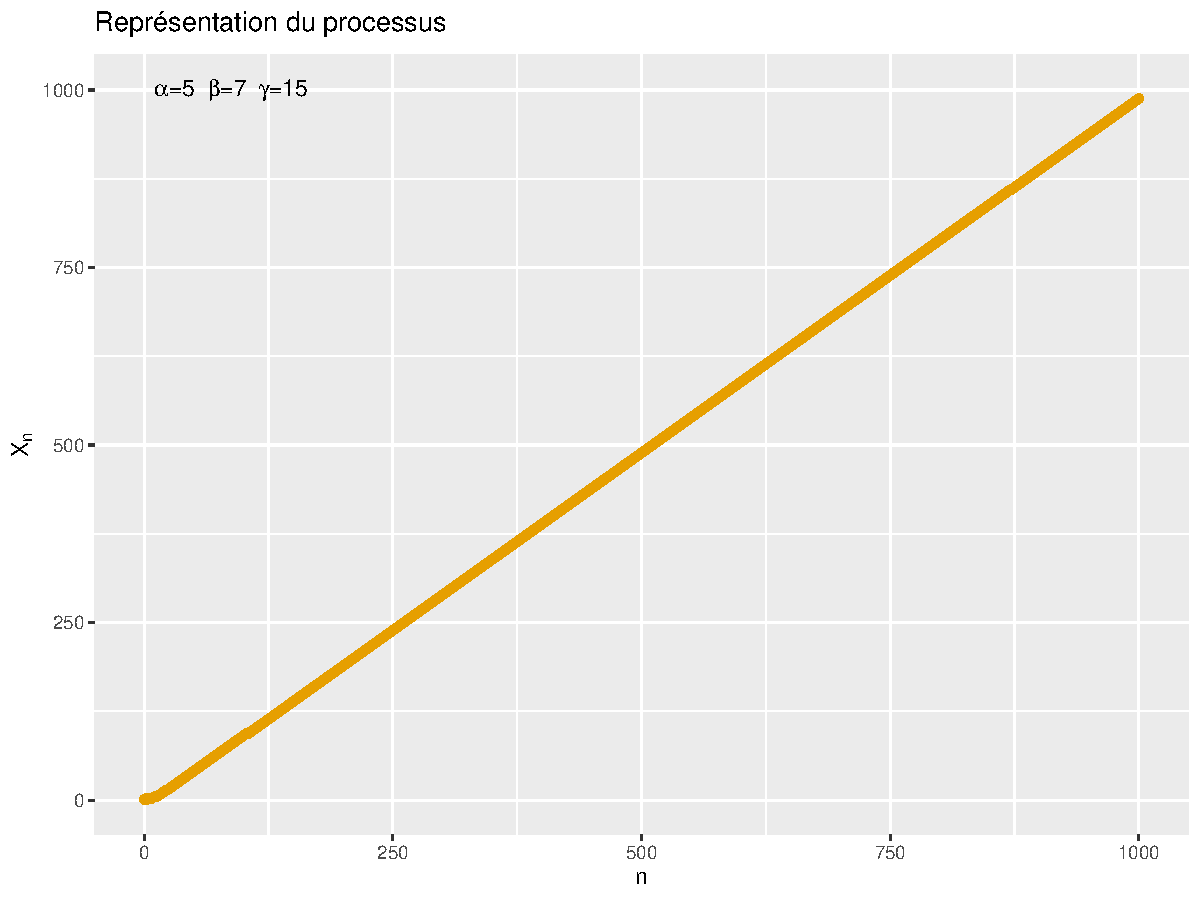
\includegraphics[scale=0.45]{mod_abs5_7_15.pdf}
    \end{minipage}
    \hfill%
    \vspace{0.1cm}
    \begin{minipage}[c]{0.50\linewidth}
        \centering
       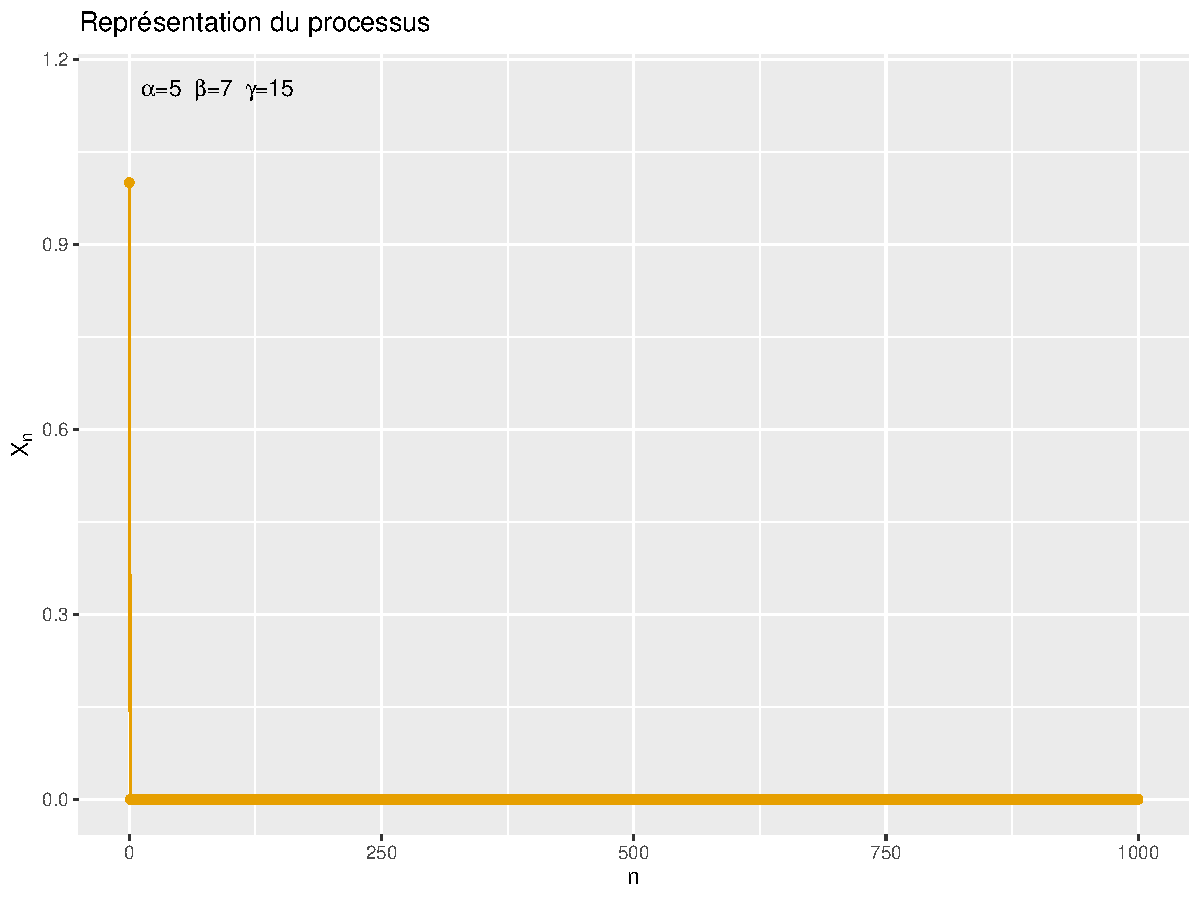
\includegraphics[scale=0.45]{mod_abs5_7_15(2).pdf}
    \end{minipage}
    \caption{Représentation du processus pour le modèle de contamination}
    \label{modele_conta}
\end{figure} 

Dans ce modèle-ci, $X_0 =1$ et bien que les paramètres soient identiques, nous observons dans la figure \ref{modele_conta} deux courbes totalement différentes. Cela est dû au comportement aléatoire de la chaîne. En effet, sur le graphique de gauche, le nombre de contaminés tend vers $+\infty$ et il n'y a aucun retour en $0$, ce qui est cohérent avec la limite trouvée précédemment. Le graphique de droite représente la seconde possibilité où l'état $0$ est atteint et l'épidémie est éteinte. Notons que $0$ est atteint très rapidement. En effet, la plus grande probabilité de l'atteindre en temps fini est celle partant de l'état $1$. Cette probabilité ne faisant que décroître en fonction du nombre de contaminés pour tendre vers $0$, il est donc normal d'atteindre l'état $0$ en un temps très court.

\vspace{1.5cm}
En conclusion, les deux modèles, contamination et guérison, ont des comportements en temps long bien différents. En effet, lorsque le modèle dépend de la guérison, l‘épidémie retourne continuellement en zéro. De plus, un taux de guérison élevé entraîne un retour en zéro d’autant plus fréquent.
A contrario, lorsque la modélisation dépend de la contamination, la chaîne de Markov admet deux classes. Les deux comportements suivants de l’épidémie sont donc possibles. Dans un cas, l’épidémie retourne rapidement  en zéro et y reste. Ceci est du à la nature absorbante de la classe. L’épidémie est ainsi rapidement contrôlée. Dans le second cas, en revanche, on voit l’épidémie se propager indéfiniment. Plus cette dernière se propage, plus la probabilité de guérison est faible. De ce fait, l’épidémie devient alors incontrôlable. Ces deux modèles permettent une représentation plus proche de la réalité que le modèle simple. Maintenant que nous avons pu voir l'implication des paramètres dans les modèles, nous allons chercher à les estimer dans le chapitre suivant.

\newpage
\chapter{Statistiques de chaînes de Markov}

\section{Estimateurs par la matrice de transition}
\vspace{0.6cm}

Dans cette partie, nous nous plaçons de nouveau dans le modèle de guérison de la section $2.1$, dans le cas où la chaîne est récurrente positive. Notre objectif va être d'estimer les paramètres $\alpha$, $\beta$ et $\gamma$ à partir des estimateurs des coefficients de la matrice de transition. Le problème est que nous obtenons les mêmes probabilités en multipliant $\alpha$, $\beta$ et $\gamma$ par une même constante. Il est donc impossible de déterminer directement les estimateurs $\hat{\alpha}$, $\hat{\beta}$ et $\hat{\gamma}$. Pour remédier à cela, nous devons choisir arbitrairement une valeur pour un des paramètres. Nous prenons : $\beta = 1$. Les taux de guérison et contamination seront donc les paramètres à estimer.

\begin{thm}\label{expression_alpha_gamma}
Les estimateurs des paramètres $\alpha$ et $\gamma$ peuvent s'écrire de la manière suivante pour $n \in \mathbb{N}$ assez grand : \\
\begin{itemize}
    \item $\hat{\alpha^n} =\frac{\hat{p_{00}}^n- \hat{p_{11}}^n}{\hat{p_{00}}^n\hat{p_{11}}^n},$\\
    \item $\hat{\gamma^n} =\frac{1-\hat{p_{00}}^n}{\hat{p_{00}}^n}.$
\end{itemize}
\end{thm}

\begin{proof}
Tout d'abord, exprimons $\alpha$ et $\gamma$ en fonction des coefficients $p_{00}$ et $p_{11}$ de la matrice de transition du modèle de guérison.
On a le système suivant :

\begin{align*}
(S') : &\left\{
\begin{array}{ll}
        p_{00} = \frac{\beta}{\beta+\gamma} \\
        p_{11} = \frac{\beta}{\alpha+\beta+\gamma} 
    \end{array}
\right.
\iff\left\{
\begin{array}{ll}
          p_{00} = \frac{1}{1+\gamma} \\
        p_{11} = \frac{1}{\alpha+1+\gamma}
    \end{array}
\right.
\iff \left\{
\begin{array}{ll}
         p_{00}(1+\gamma)= 1 \\
        p_{11}(\alpha + 1 +\gamma) =1  \end{array}
\right.\\
\iff &\left\{
\begin{array}{ll}
          p_{00}\gamma= 1-p_{00} \\
        p_{11}\alpha = 1 - p_{11}(1+\gamma)   \end{array}
    \right.
\iff \left\{
\begin{array}{ll}
        \gamma= \frac{1-p_{00}}{p_{00}} \\
       p_{11}\alpha = 1 - p_{11}(1+\frac{1-p_{00}}{p_{00}})  
       \end{array}  
    \right.   
\iff \left\{
\begin{array}{ll}
         \gamma= \frac{1-p_{00}}{p_{00}} \\
        \alpha = \frac{p_{00}-p_{11}}{p_{11}p_{00}}   
    \end{array}    
    \right.      
\end{align*}

D'après la proposition \ref{prop0}, $\forall (i,j) \in \mathbb{N}^2$ : $$\hat{p_{ij}}^n = \frac{\sum\limits_{k=0}^{n-1} \mathds{1}(X_k=i, X_{k+1}=j)}{\sum\limits_{k=0}^{n-1} \mathds{1}(X_k=i)} \, \, \, \text{ est un estimateur convergent de } p_{ij}.$$

On en déduit les estimateurs de $\alpha$ et $\gamma$.
\begin{align*}
\hat{\alpha}^n &= \frac{\hat{p_{00}}^n-\hat{p_{11}}^n}{\hat{p_{00}}^n\hat{p_{11}}^n} \\
&= \frac{\sum\limits_{k=0}^{n-1} \mathds{1}(X_k=0, X_{k+1}=0)\sum\limits_{k=0}^{n-1} \mathds{1}(X_k=1)-\sum\limits_{k=0}^{n-1} \mathds{1}(X_k=1, X_{k+1}=1)\sum\limits_{k=0}^{n-1} \mathds{1}(X_k=0)}{\sum\limits_{k=0}^{n-1} \mathds{1}(X_k=0, X_{k+1}=0)\sum\limits_{k=0}^{n-1} \mathds{1}(X_k=1, X_{k+1}=1)}\\
\hat{\gamma}^n &= \frac{1- \hat{p_{00}}^n}{\hat{p_{00}}^n} \\
&= \frac{{\sum\limits_{k=0}^{n-1} \mathds{1}(X_k=0)}}{{\sum\limits_{k=0}^{n-1} \mathds{1}(X_k=0,X_{k+1}=0)}} - 1
\end{align*}
\end{proof}

\begin{remark}
Calculer les estimateurs de $\alpha$ et $\gamma$ par la loi invariante nous donne un modèle multiplicatif qui ne dépend pas de $\beta$. Cela rend leurs analyses peu pertinentes puisque nous serions obligés de poser un paramètre supplémentaire.
\end{remark}

\section{Convergence des estimateurs}

\vspace{0.6cm}
\begin{prop}\label{prop_conv}
Les estimateurs $\hat{\alpha_n}$ et $\hat{\gamma_n}$ sont des estimateurs convergents respectivement de $\alpha$ et $\gamma$ :
$$\lim\limits_{n \to +\infty}\hat{\alpha^n} =\alpha \, \, \, \text{ et } \, \, \, \lim\limits_{n \to +\infty}\hat{\gamma^n} =\gamma.$$
\end{prop}

\begin{proof}
D'après la proposition \ref{prop0} , on sait que $\hat{p_{ij}}^n$ est un estimateur convergent de $p_{ij}$, c'est-à-dire que $\forall (i,j) \in \mathbb{N}^2$: 
$$\lim\limits_{n \to +\infty}\hat{p_{ij}}^n = p_{ij}.$$ 

D'où, par somme et produit : \\
\begin{itemize}
    \item $\lim\limits_{n \to +\infty}\hat{\alpha^n} =\lim\limits_{n \to +\infty}\frac{\hat{p_{00}}^n-\hat{p_{11}}^n}{\hat{p_{00}}^n\hat{p_{11}}^n} = \frac{p_{00}-p_{11}}{p_{00}p_{11}} = \alpha .$\\
    \item $\lim\limits_{n \to +\infty}\hat{\gamma^n} = \lim\limits_{n \to +\infty}\frac{1-\hat{p_{00}}^n}{\hat{p_{00}}^n} =\frac{1-p_{00}}{p_{00}}= \gamma .$
\end{itemize}
\end{proof}

\begin{remark}
Il se trouve que les estimateurs $\hat{p_{ij}}^n$ coïncident avec les estimateurs de maximum de vraisemblance. Pour plus de détails, voir \cite{cle4}.
\end{remark}

\begin{example}\label{exemple_convergence}
Afin d'illustrer la convergence des estimateurs de $\alpha$ et $\gamma$, nous avons simulé une chaîne de Markov de paramètres $\alpha =15, \beta = 1$ et $\gamma =10$ avec $n=100 000$.

\begin{figure}[h]
 \begin{minipage}[c]{0.25\linewidth}
        \centering
        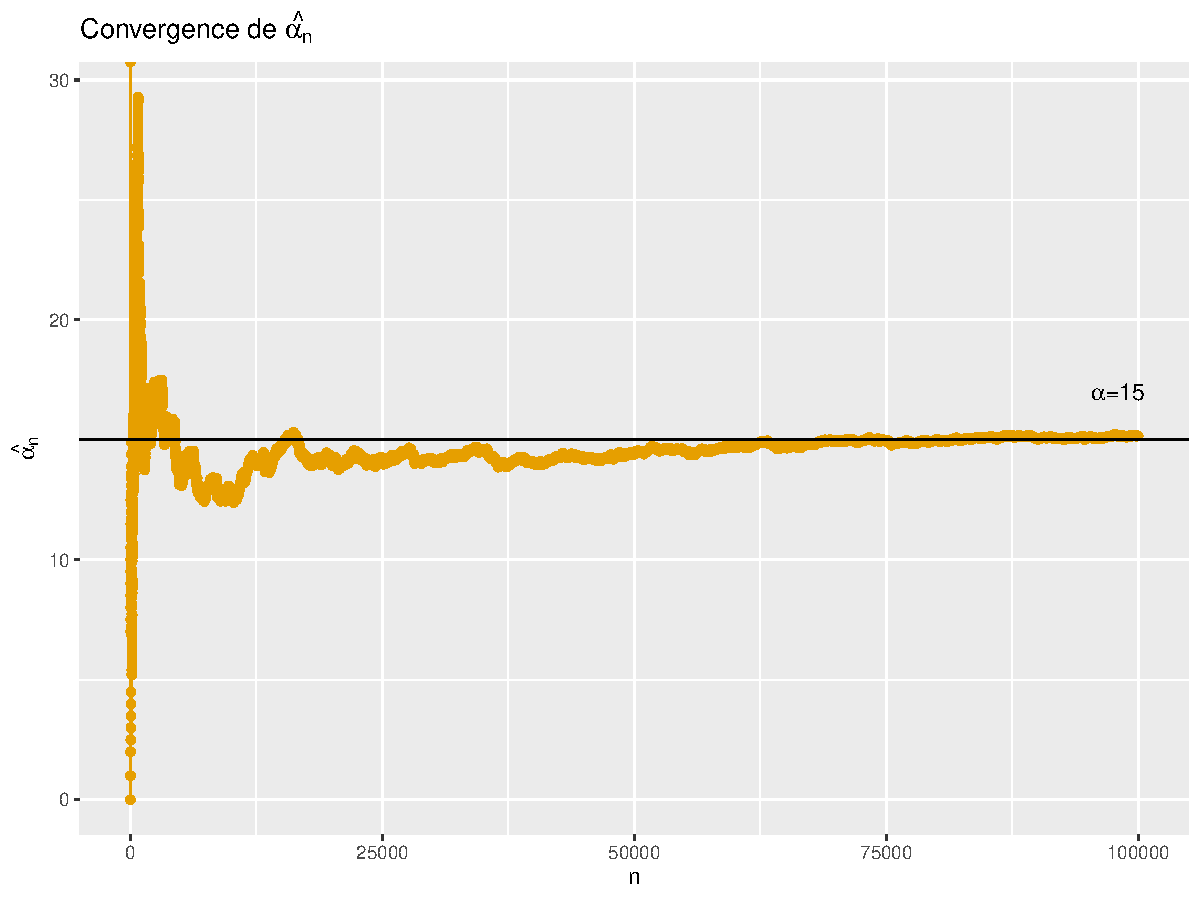
\includegraphics[scale=0.45]{convergence_alpha.pdf}
    \end{minipage}
    \hfill%
    \vspace{0.1cm}
    \begin{minipage}[c]{0.50\linewidth}
        \centering
       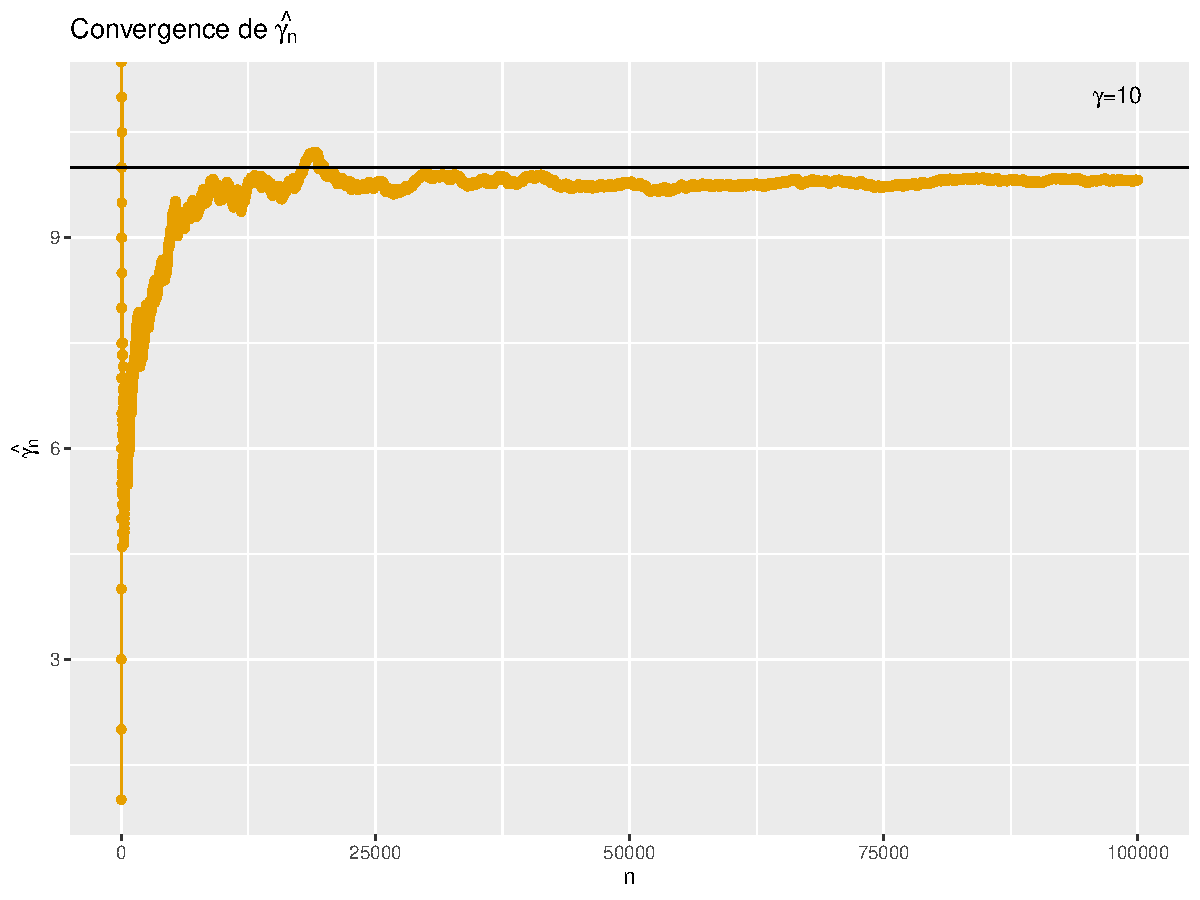
\includegraphics[scale=0.45]{convergence_gamma.pdf}
    \end{minipage}
    \caption{Convergence des estimateurs de $\alpha$ et $\gamma$ respectivement}
    \label{convergence}
\end{figure}

Nous remarquons que les estimateurs tendent vers la valeur que nous avons fixé. En effet, les estimateurs convergent vers leurs "vrais" valeurs prédéfinies lorsque $n$ est suffisamment grand.
\end{example}

\newpage
\section{Loi des estimateurs}
\vspace{0.6cm}

Nous souhaitons à présent déterminer la loi des estimateurs de $\alpha$ et $\gamma$.
Pour ce faire, nous simulons 100 fois le même modèle, avec $n=100 000, \alpha=15, \beta=1$ et $\gamma=10$. Nous calculons nos estimateurs en temps long et obtenons les graphiques de la figure \ref{hist}.

\begin{figure}[h]
 \begin{minipage}[c]{0.25\linewidth}
        \centering
        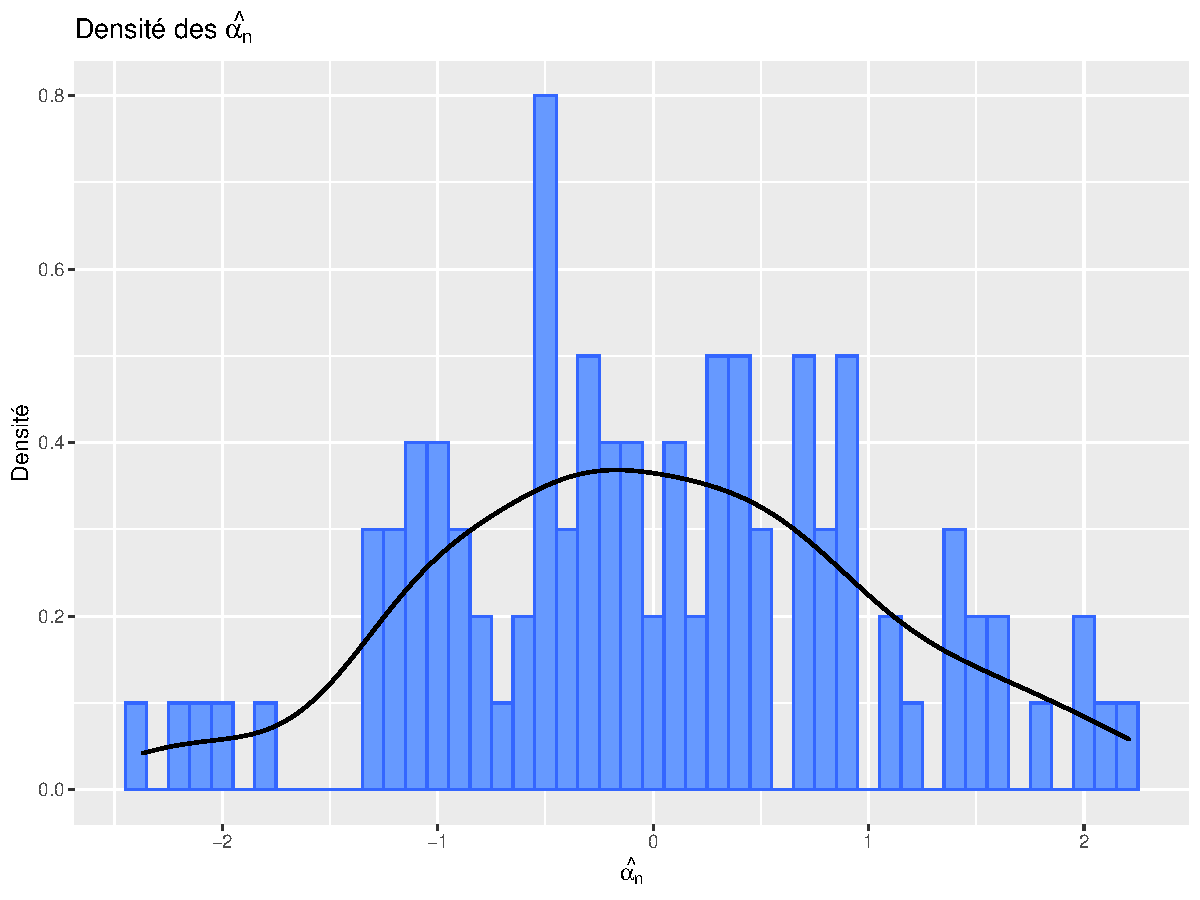
\includegraphics[scale=0.45]{densite_alpha_2.pdf}
    \end{minipage}
    \hfill%
    \vspace{0.1cm}
    \begin{minipage}[c]{0.50\linewidth}
        \centering
       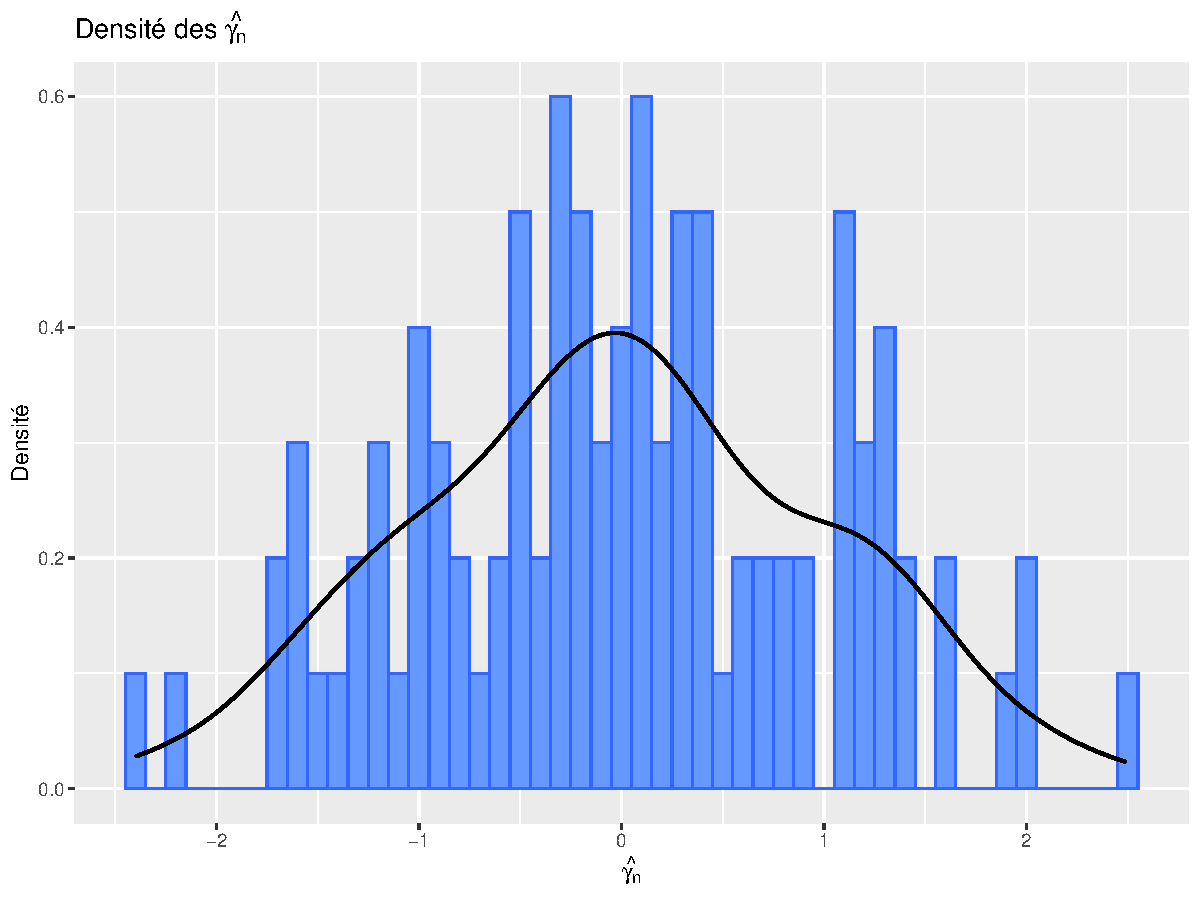
\includegraphics[scale=0.45]{densite_gamma_2.pdf}
    \end{minipage}
    \caption{Histogramme de densité des estimateurs de $\alpha$ et $\gamma$ respectivement}
    \label{hist}
\end{figure}

Les données représentés à l'aide des histogrammes de fréquence semblent s'ajuster à une distribution normale. De ce fait, nous souhaitons vérifier la normalité de nos estimateurs. \\
\\
Pour cela, nous allons appliquer le  test de Shapiro-Wilk. Ce dernier  teste l'hypothèse $H_0$: "L'estimateur suit une loi Normale" contre l'hypothèse $H_1$: "L'estimateur ne suit pas une loi Normale". Rappelons que $H_0$ est rejeté si la p-value est plus petite que $\alpha=0,05$. 
\newpage
\begin{figure}[h!]
 \begin{minipage}[c]{0.25\linewidth}
        \centering
        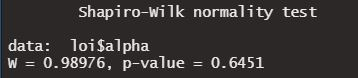
\includegraphics[scale=1.10]{shapiro_alpha2.JPG}
    \end{minipage}
    \hfill%
    \vspace{0.1cm}
    \begin{minipage}[c]{0.50\linewidth}
        \centering
       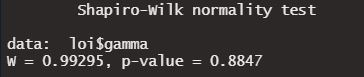
\includegraphics[scale=1.10]{shapiro_gamma2.JPG}
    \end{minipage}
    \caption{Test de Shapiro-Wilk des estimateurs de $\alpha$ et $\gamma$ respectivement}

\end{figure}

Les $p$-values de nos deux estimateurs $\hat{\alpha^n}$ et $\hat{\gamma^n}$ sont très élevées. On ne rejette donc pas l'hypothese de normalité des coefficients au risque $5 \%$. Ainsi, quand $n$ est suffisamment grand, $\hat{\alpha^n}$ et $\hat{\gamma^n}$ suivent des lois normales.


\newpage
\section*{Conclusion}
\vspace{0.6cm}

Les travaux présentés ont eu pour but de modéliser la propagation d'une épidémie et d’estimer au mieux les paramètres qui la contrôlent. Dans un premier temps, nous avons défini et étudié un modèle simple, où les probabilités de contamination, infection et inaction ont été posées de manière constante. Dans un second temps, nous avons complexifié les modèles, en renforçant tout d’abord la probabilité de guérison, puis celle de  contamination. L’analyse des différents modèles nous a permis de mettre en évidence des résultats intéressants, et d’anticiper le comportement en temps long de nos modèles selon les différentes valeurs des paramètres. Pour mieux visualiser les dynamiques de nos modèles et l’influence des paramètres, nous avons simulé certains cas. Enfin, pour finir,  nous avons cherché à estimer les paramètres de la section 2.1 et analyser leurs caractéristiques.
\\
\\
Ce projet a été pour nous très enrichissant. Il nous a permis d’approfondir d’avantage les notions déjà traités en cours. Néanmoins, le travail fourni n’a pas toujours été facile. Nous avons été surpris par l'aspect calculatoire du projet. Nous avons passé beaucoup de temps aux résolutions de systèmes. Le deuxième obstacle auquel nous avons été confronté a été les estimateurs. Vu que nous avancions en terre inconnue, nous avons parfois chercher à estimer les paramètres par des méthodes qui étaient impossibles ou peu pertinentes. C’est pourquoi il a été nécessaire de fixer le paramètre $\beta$ afin de trouver les estimateurs par la matrice de transition. Nous avons passé beaucoup de temps à simuler nos résultats dans le but de trouver des conjectures. De plus, très peu de documentations étaient appropriées à nos besoins. Notez que nous avons rendu disponible nos programmes entièrement paramétrables sur le compte GitHub suivant :  
\begin{center}
    \url{https://github.com/Assiab2707/projet_modeles_epidemies}
\end{center}

La modélisation de la propagation d’une épidémie est un moyen de distinguer les cas où l’épidémie s’étendra de ceux où elle s’éteindra, et permet donc de faciliter la prise de décision. Néanmoins, dans des modèles plus réalistes, prenant en compte la complexité des interactions entre individus par exemple, nos modèles « naïfs » ne suffisent plus. Il faudrait ainsi réfléchir à des modèles plus pertinents. La difficulté est alors de déterminer les hypothèses d’un modèle afin qu’il soit adaptée au mieux à la situation. Par conséquent, des extensions de nos modèles peuvent être trouver afin d’y apporter de nouvelles perspectives. En effet, il aurait été intéressant de se placer dans un espace d’état fini. Nous aurions pu également admettre, dans ce cas, qu’un individu guéri est immunisé. L’étude en temps long aurait été différente et nous aurions pu nous demander sous quelle conditions notre population aurait connu l’immunité collective. Finalement, les modèles que nous avons étudié sont efficaces dans certaines situations, mais restent perfectibles.


\begin{thebibliography}{8} 
\bibitem[1]{cle1} Benoîte de Saporta,{"Chaînes de Markov",  Processus Stochastiques, \url{https://moodle.umontpellier.fr/pluginfile.php/1240925/mod_resource/content/1/Chap3-Markov.pdf}, HMMA103, 2020-2021}
\\
\\
\bibitem[2]{cle2} J-F Delams et B. Jourdain,{"Applications aux sciences de l'ingénieur et du vivant" , MATHEMATIQUES ET APPLICATIONS Comité de Lecture / Editorial Board, 2006 } 
\\
\\
\bibitem[3]{cle3} Santinelli Emma et Hanna Bacave, {"Optimisation de la gestion d'une eploitation forestière", Projet Master 1, 2020}
\\
\\
\bibitem[4]{cle4} Benoîte de Saporta,{"Statistique des Chaînes de Markov",  Université de Monastir, 2016-2017} 
\\
\\
\bibitem[5]{cle5} Statistiques des Processus 3A, {\url{http://ensai.fr/wp-content/uploads/2019/06/polystatdesprocessus2.pdf}, 2015}
\end{thebibliography}


\chapter*{Annexes}
La librairie utilisée pour l'ensemble de ces simulations est la librairie "ggplot2". Il suffit de la charger à l'aide de la commande "library(ggplot2)".

\section*{Code de la représentation du modèle simple}

\begin{lstlisting}
simu_simple<- function(H,alpha,beta,gamma){
  X<-NULL
  X[1]<-0
  proba<-c(alpha/(alpha+beta+gamma),beta/(alpha+beta+gamma)
            ,gamma/(alpha+beta+gamma))
  U<-sample(c(-1,0,1),H,replace=TRUE, prob=proba)
  for (i in 1:H){
    X[i+1]<-(X[i]+U[i])*(X[i]>0)+ (X[i]==0)*(U[i]==1)
  }
  simu<-data.frame(0:1000,X)
  colnames(simu)<-c("n","X_n")
  return(simu)
}

#Récurrente positive
simu_1<-simu_simple(1000,60,30,40)
simu_1bis<-simu_simple(1000,60,40,30)
ggplot(data=simu_1,aes(n,X_n)) + geom_line(color="#E69F00")+
    geom_point(color="#E69F00")+ylab(expression(X[n]))+ 
    ggtitle(expression(paste("Représentation du processus dans le cas 
        où ",     (X[n])[n], " est récurrente positive")))+
    annotate("text", x=100, y =17, label = 
    expression(paste(alpha,"=60    ", beta,"=30    ",gamma,"=40    ")))

ggplot(data=simu_1bis,aes(n,X_n)) + geom_line(color="#E69F00")+
    geom_point(color="#E69F00")+ylab(expression(X[n]))+
    ggtitle(expression(paste("Représentation du processus dans le cas
        où ", (X[n])[n], " est récurrente positive")))+
    annotate("text", x=100, y =6, label =
    expression(paste(alpha,"=60    ", beta,"=40    ",gamma,"=30    ")))

#Transitoire
simu_2<-simu_simple(1000,20,30,50)
simu_2bis<-simu_simple(1000,30,20,50)
ggplot(data=simu_2,aes(n,X_n)) + geom_line(color="#33CC66")+
    geom_point(color="#33CC66")+ylab(expression(X[n]))+ 
    ggtitle(expression(paste("Représentation du processus dans le cas 
        où ", (X[n])[n], " est transitoire")))+
    annotate("text", x=100, y =310, label = 
    expression(paste(alpha,"=20    ", beta,"=30    ",gamma,"=50    ")))
    
ggplot(data=simu_2bis,aes(n,X_n)) + geom_line(color="#33CC66")+
    geom_point(color="#33CC66")+ylab(expression(X[n]))+ 
    ggtitle(expression(paste("Représentation du processus dans le cas 
        où ", (X[n])[n], " est transitoire")))+
    annotate("text", x=100, y =230, label = 
    expression(paste(alpha,"=30    ", beta,"=20    ",gamma,"=50    ")))

#Récurrente nulle
simu_3<-simu_simple(1000,30,50,30)
simu_3bis<-simu_simple(1000,40,10,40)
ggplot(data=simu_3,aes(n,X_n)) + geom_line(color="#6666FF")+
    geom_point(color="#6666FF")+ylab(expression(X[n]))+ 
    ggtitle(expression(paste("Représentation du processus dans le cas
        où ", (X[n])[n], " est récurrente nulle")))+
    annotate("text", x=100, y =28, label = 
    expression(paste(alpha,"=30    ", beta,"=50    ",gamma,"=30    ")))

ggplot(data=simu_3bis,aes(n,X_n)) + geom_line(color="#6666FF")+
    geom_point(color="#6666FF")+ylab(expression(X[n]))+ 
    ggtitle(expression(paste("Représentation du processus dans le cas 
        où ", (X[n])[n], " est récurrente nulle")))+
    annotate("text", x=100, y =33, label =
    expression(paste(alpha,"=40    ", beta,"=10    ",gamma,"=40    ")))
\end{lstlisting}

\section*{Code de la représentation du modèle de guérison}
\begin{lstlisting}
N=1000
simu_guerison<- function(H,alpha,beta,gamma){
  X<-NULL
  X[1]<-1
  for (i in 1:H){
    proba<-c(X[i]*alpha/(X[i]*alpha+beta+gamma),
            beta/(X[i]*alpha+beta+gamma)
            ,gamma/(X[i]*alpha+beta+gamma))
    U<-sample(c(-1,0,1),H,replace=TRUE, prob=proba)
    X[i+1]<-(X[i]+U[i])*(X[i]>0)+ (X[i]==0)*(U[i]==1)
  }
  simu<-data.frame(0:1000,X)
  colnames(simu)<-c("n","X_n")
  return(simu)
}

simu_gueri1<-simu_guerison(N,10,30,50)
ggplot(data=simu_gueri1,aes(n,X_n)) + geom_line(color="#E69F00")+
    geom_point(color="#E69F00")+ylab(expression(X[n]))+ 
    ggtitle(expression(paste("Représentation du processus ", (X[n])[n])))+
    annotate("text", x=100, y =12, label = 
    expression(paste(alpha,"=10    ", beta,"=30    ",gamma,"=50    ")))

simu_gueri2<-simu_guerison(N,15,10,10)
ggplot(data=simu_gueri2,aes(n,X_n)) + geom_line(color="#E69F00")+
    geom_point(color="#E69F00")+ylab(expression(X[n]))+ 
    ggtitle(expression(paste("Représentation du processus ", (X[n])[n])))+
    annotate("text", x=100, y =5.3, label = 
    expression(paste(alpha,"=15    ", beta,"=10    ",gamma,"=10    ")))
\end{lstlisting}

\section*{Code de la représentation du modèle de contamination}

\begin{lstlisting}
N=1000
model_contamination<- function(H,alpha,beta,gamma){
  X<-NULL
  X[1]<-1
  for (i in 1:H){
    proba<-c(alpha/(alpha+beta+X[i]*gamma),
            beta/(alpha+beta+X[i]*gamma),
            (X[i]*gamma)/(alpha+beta+X[i]*gamma))
    U<-sample(c(-1,0,1),H,replace=TRUE, prob=proba)
    X[i+1]<-(X[i]+U[i])*(X[i]>0)+ (X[i]==0)*(U[i]==1)
  }
  simu<-data.frame(0:1000,X)
  colnames(simu)<-c("n","X_n")
  return(simu)
}
simu_conta1<-model_contamination(N,5,7,8)
ggplot(data=simu_conta1,aes(n,X_n)) + geom_line(color="#E69F00")+
    geom_point(color="#E69F00")+ ylab(expression(X[n]))+ 
    ggtitle(expression(paste("Représentation du processus")))+
    annotate("text", x=100, y =1.15, label = 
    expression(paste(alpha,"=5  ", beta,"=7  ",gamma,"=15    ")))

simu_conta2<-model_contamination(N,5,7,15)
ggplot(data=simu_conta2,aes(n,X_n)) +geom_line(color="#E69F00")+
    geom_point(color="#E69F00")+ylab(expression(X[n]))+
    ggtitle(expression(paste("Représentation du processus")))+
    annotate("text", x=100, y =1000, label =
    expression(paste(alpha,"=5  ", beta,"=7  ",gamma,"=15    ")))
\end{lstlisting}

\section*{Code simulant les estimateurs et leurs comportements}
\begin{lstlisting}
N=100000
alpha = 15
gamma = 10

#Estimateurs
simu_contamination_estimateur<- function(H,alpha,gamma){
  beta<-1
  X<-NULL
  X[1]<-0
  for (i in 1:H){
    proba<-c(X[i]*alpha/(X[i]*alpha+beta+gamma),
        beta/(X[i]*alpha+beta+gamma),
        gamma/(X[i]*alpha+beta+gamma))
    U<-sample(c(-1,0,1),H,replace=TRUE, prob=proba)
    X[i+1]<-(X[i]+U[i])*(X[i]>0)+ (X[i]==0)*(U[i]==1)
  }
  return(X)
}
mod1<-simu_contamination_estimateur(N,alpha,gamma)
plot(mod1,type="o",col="blue",xlab='n',ylab=expression(X[n]), pch=16)

pij_hat<- function(simu,n,i,j){
  p_ij<-NULL
  num<-0
  denum<-0
  for (k in 1:n){
    num<- num+as.numeric(simu[k]==i && simu[k+1]==j)
    denum<- denum + (as.numeric(simu[k]==i))
    p_ij[k]<- num/denum
  }
  return(p_ij)
}

p_00<- pij_hat(mod1,N,0,0)
plot(p_00,type="o",col="blue",xlab='n',ylab=expression(p["00"]), pch=16)
abline(h=1/(1+gamma))

p_11<- pij_hat(mod1,N,1,1)
plot(p_11,type="o",col="blue",xlab='n',ylab=expression(p["11"]), pch=16)
abline(h=1/(alpha+1+gamma))



alpha_hat<- function(hat_p00, hat_p11){
  alpha_n_hat<-NULL
  for (i in 1:length(hat_p00)){
    alpha_n_hat[i]<- (hat_p00[i]-hat_p11[i])/(hat_p00[i]*hat_p11[i])
  }
  simu_alpha<-data.frame(0:(length(hat_p00)-1),alpha_n_hat)
  colnames(simu_alpha)<-c("n","h_alpha")
  return(simu_alpha)
}

alpha_n<- alpha_hat(p_00, p_11)
ggplot(data=alpha_n,aes(n,h_alpha)) + geom_line(color="#E69F00")+
    geom_point(color="#E69F00")+ylab(expression(hat(alpha[n])))+
    ggtitle(expression(paste("Convergence de ", hat(alpha[n]))))+
    annotate("text", x=98000, y =17, label = 
    expression(paste(alpha,"=15")))+geom_hline(yintercept=alpha)

gamma_hat<- function(hat_p00, hat_p11){
  gamma_n_hat<-NULL
  for (i in 1:length(hat_p00)){
    gamma_n_hat[i]<- (1-hat_p00[i])/(hat_p00[i])
  }
  simu_gamma<-data.frame(0:(length(hat_p00)-1),gamma_n_hat)
  colnames(simu_gamma)<-c("n","h_gamma")
  return(simu_gamma)
}
gamma_n<- gamma_hat(p_00, p_11)
ggplot(data=gamma_n,aes(n,h_gamma)) + geom_line(color="#E69F00")+
    geom_point(color="#E69F00")+ylab(expression(hat(gamma[n])))+
    ggtitle(expression(paste("Convergence de ", hat(gamma[n]))))+
    annotate("text", x=98000, y =11, label =
    expression(paste(gamma,"=10")))+geom_hline(yintercept=gamma)


#Loi estimateurs
loi_estimateur<-function(H, al,gam, nbsimu){
  tab_gamma<-NULL
  tab_alpha<-NULL
  for (i in 1:nbsimu){
    simu<- simu_contamination_estimateur(H,al,gam)
    p_00<- pij_hat(simu,H,0,0)
    p_11<- pij_hat(simu,H,1,1)
    tab_alpha[i]<- alpha_hat(p_00, p_11)$h_alpha[H]
    tab_gamma[i]<- gamma_hat(p_00, p_11)$h_gamma[H]
  }
  return(data.frame(alpha=tab_alpha,gamma=tab_gamma))
}

loi<- loi_estimateur(100000,alpha,gamma,100)
ggplot(loi, aes(x = scale(alpha))) +
  geom_histogram(aes(y = ..density..), binwidth = 0.1,
                 colour = "#3366FF", fill = "#6699FF") + 
  geom_density(size = 0.8, alpha = 0.05) +
  scale_x_continuous(name = expression(hat(alpha[n])))+
  scale_y_continuous(name = "Densité") +
  ggtitle(expression(paste("Densité des ", hat(alpha[n]))))

ggplot(loi, aes(x = scale(gamma))) +
  geom_histogram(aes(y = ..density..), binwidth = 0.1,
                 colour = "#3366FF", fill = "#6699FF") + 
  geom_density(size = 0.8, alpha = 0.05) +
  scale_x_continuous(name = expression(hat(gamma[n])))+
  scale_y_continuous(name = "Densité") +
  ggtitle(expression(paste("Densité des ", hat(gamma[n]))))

#Test de Shapiro-Wilk
shapiro.test(loi$alpha)
shapiro.test(loi$gamma)
 
\end{lstlisting}

\end{document}
